% Created by tikzDevice version 0.12.6 on 2024-08-29 11:34:31
% !TEX encoding = UTF-8 Unicode
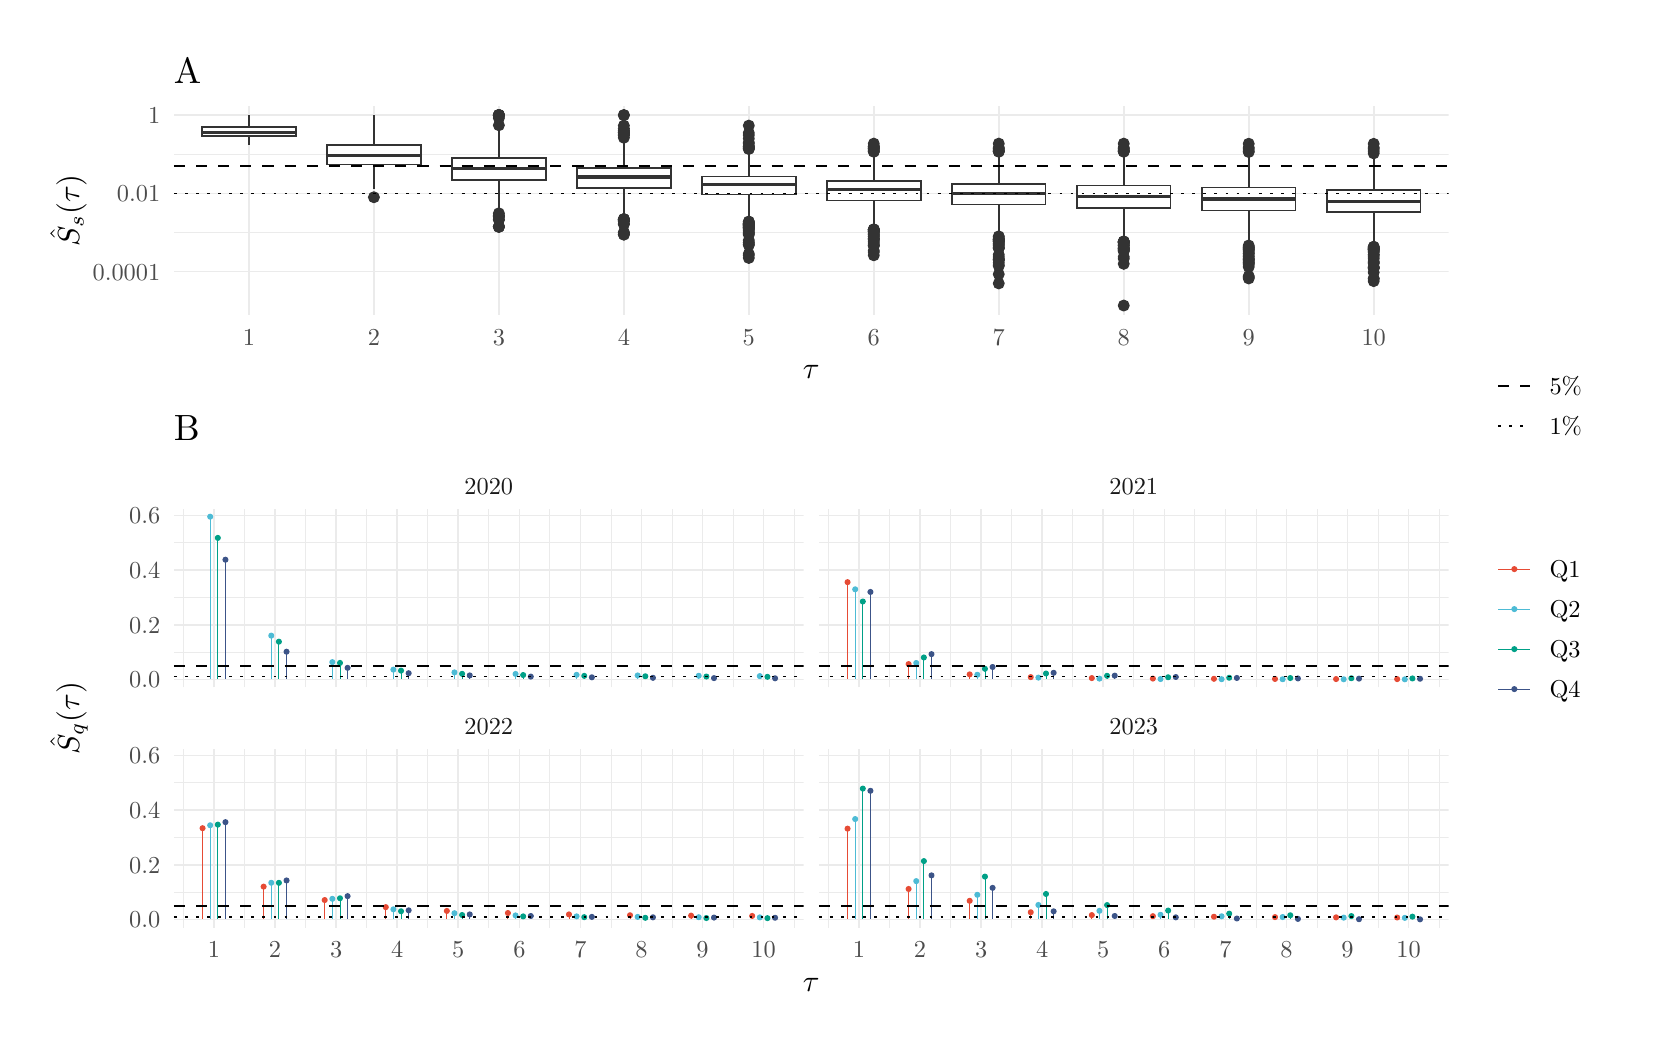
\begin{tikzpicture}[x=1pt,y=1pt]
\definecolor{fillColor}{RGB}{255,255,255}
\path[use as bounding box,fill=fillColor,fill opacity=0.00] (0,0) rectangle (578.16,361.35);
\begin{scope}
\path[clip] ( 52.85,257.50) rectangle (513.48,333.19);
\definecolor{drawColor}{gray}{0.92}

\path[draw=drawColor,line width= 0.3pt,line join=round] ( 52.85,315.61) --
	(513.48,315.61);

\path[draw=drawColor,line width= 0.3pt,line join=round] ( 52.85,287.33) --
	(513.48,287.33);

\path[draw=drawColor,line width= 0.6pt,line join=round] ( 52.85,329.75) --
	(513.48,329.75);

\path[draw=drawColor,line width= 0.6pt,line join=round] ( 52.85,301.47) --
	(513.48,301.47);

\path[draw=drawColor,line width= 0.6pt,line join=round] ( 52.85,273.19) --
	(513.48,273.19);

\path[draw=drawColor,line width= 0.6pt,line join=round] ( 79.95,257.50) --
	( 79.95,333.19);

\path[draw=drawColor,line width= 0.6pt,line join=round] (125.11,257.50) --
	(125.11,333.19);

\path[draw=drawColor,line width= 0.6pt,line join=round] (170.27,257.50) --
	(170.27,333.19);

\path[draw=drawColor,line width= 0.6pt,line join=round] (215.43,257.50) --
	(215.43,333.19);

\path[draw=drawColor,line width= 0.6pt,line join=round] (260.58,257.50) --
	(260.58,333.19);

\path[draw=drawColor,line width= 0.6pt,line join=round] (305.74,257.50) --
	(305.74,333.19);

\path[draw=drawColor,line width= 0.6pt,line join=round] (350.90,257.50) --
	(350.90,333.19);

\path[draw=drawColor,line width= 0.6pt,line join=round] (396.06,257.50) --
	(396.06,333.19);

\path[draw=drawColor,line width= 0.6pt,line join=round] (441.22,257.50) --
	(441.22,333.19);

\path[draw=drawColor,line width= 0.6pt,line join=round] (486.38,257.50) --
	(486.38,333.19);
\definecolor{drawColor}{gray}{0.20}

\path[draw=drawColor,line width= 0.6pt,line join=round] ( 79.95,325.40) -- ( 79.95,329.75);

\path[draw=drawColor,line width= 0.6pt,line join=round] ( 79.95,322.27) -- ( 79.95,319.12);
\definecolor{fillColor}{RGB}{255,255,255}

\path[draw=drawColor,line width= 0.6pt,fill=fillColor] ( 63.01,325.40) --
	( 63.01,322.27) --
	( 96.88,322.27) --
	( 96.88,325.40) --
	( 63.01,325.40) --
	cycle;

\path[draw=drawColor,line width= 1.1pt] ( 63.01,323.63) -- ( 96.88,323.63);
\definecolor{fillColor}{gray}{0.20}

\path[draw=drawColor,line width= 0.4pt,line join=round,line cap=round,fill=fillColor] (125.11,300.07) circle (  1.96);

\path[draw=drawColor,line width= 0.6pt,line join=round] (125.11,319.05) -- (125.11,329.75);

\path[draw=drawColor,line width= 0.6pt,line join=round] (125.11,311.87) -- (125.11,303.04);
\definecolor{fillColor}{RGB}{255,255,255}

\path[draw=drawColor,line width= 0.6pt,fill=fillColor] (108.17,319.05) --
	(108.17,311.87) --
	(142.04,311.87) --
	(142.04,319.05) --
	(108.17,319.05) --
	cycle;

\path[draw=drawColor,line width= 1.1pt] (108.17,315.23) -- (142.04,315.23);
\definecolor{fillColor}{gray}{0.20}

\path[draw=drawColor,line width= 0.4pt,line join=round,line cap=round,fill=fillColor] (170.27,293.25) circle (  1.96);

\path[draw=drawColor,line width= 0.4pt,line join=round,line cap=round,fill=fillColor] (170.27,291.85) circle (  1.96);

\path[draw=drawColor,line width= 0.4pt,line join=round,line cap=round,fill=fillColor] (170.27,289.53) circle (  1.96);

\path[draw=drawColor,line width= 0.4pt,line join=round,line cap=round,fill=fillColor] (170.27,289.45) circle (  1.96);

\path[draw=drawColor,line width= 0.4pt,line join=round,line cap=round,fill=fillColor] (170.27,293.33) circle (  1.96);

\path[draw=drawColor,line width= 0.4pt,line join=round,line cap=round,fill=fillColor] (170.27,289.36) circle (  1.96);

\path[draw=drawColor,line width= 0.4pt,line join=round,line cap=round,fill=fillColor] (170.27,294.26) circle (  1.96);

\path[draw=drawColor,line width= 0.4pt,line join=round,line cap=round,fill=fillColor] (170.27,293.01) circle (  1.96);

\path[draw=drawColor,line width= 0.4pt,line join=round,line cap=round,fill=fillColor] (170.27,293.38) circle (  1.96);

\path[draw=drawColor,line width= 0.4pt,line join=round,line cap=round,fill=fillColor] (170.27,289.39) circle (  1.96);

\path[draw=drawColor,line width= 0.4pt,line join=round,line cap=round,fill=fillColor] (170.27,292.10) circle (  1.96);

\path[draw=drawColor,line width= 0.4pt,line join=round,line cap=round,fill=fillColor] (170.27,328.67) circle (  1.96);

\path[draw=drawColor,line width= 0.4pt,line join=round,line cap=round,fill=fillColor] (170.27,329.75) circle (  1.96);

\path[draw=drawColor,line width= 0.4pt,line join=round,line cap=round,fill=fillColor] (170.27,329.74) circle (  1.96);

\path[draw=drawColor,line width= 0.4pt,line join=round,line cap=round,fill=fillColor] (170.27,326.09) circle (  1.96);

\path[draw=drawColor,line width= 0.4pt,line join=round,line cap=round,fill=fillColor] (170.27,329.75) circle (  1.96);

\path[draw=drawColor,line width= 0.4pt,line join=round,line cap=round,fill=fillColor] (170.27,329.75) circle (  1.96);

\path[draw=drawColor,line width= 0.4pt,line join=round,line cap=round,fill=fillColor] (170.27,329.75) circle (  1.96);

\path[draw=drawColor,line width= 0.4pt,line join=round,line cap=round,fill=fillColor] (170.27,329.75) circle (  1.96);

\path[draw=drawColor,line width= 0.4pt,line join=round,line cap=round,fill=fillColor] (170.27,329.75) circle (  1.96);

\path[draw=drawColor,line width= 0.4pt,line join=round,line cap=round,fill=fillColor] (170.27,329.75) circle (  1.96);

\path[draw=drawColor,line width= 0.6pt,line join=round] (170.27,314.22) -- (170.27,325.96);

\path[draw=drawColor,line width= 0.6pt,line join=round] (170.27,306.33) -- (170.27,294.51);
\definecolor{fillColor}{RGB}{255,255,255}

\path[draw=drawColor,line width= 0.6pt,fill=fillColor] (153.33,314.22) --
	(153.33,306.33) --
	(187.20,306.33) --
	(187.20,314.22) --
	(153.33,314.22) --
	cycle;

\path[draw=drawColor,line width= 1.1pt] (153.33,310.34) -- (187.20,310.34);
\definecolor{fillColor}{gray}{0.20}

\path[draw=drawColor,line width= 0.4pt,line join=round,line cap=round,fill=fillColor] (215.43,292.12) circle (  1.96);

\path[draw=drawColor,line width= 0.4pt,line join=round,line cap=round,fill=fillColor] (215.43,290.30) circle (  1.96);

\path[draw=drawColor,line width= 0.4pt,line join=round,line cap=round,fill=fillColor] (215.43,291.56) circle (  1.96);

\path[draw=drawColor,line width= 0.4pt,line join=round,line cap=round,fill=fillColor] (215.43,286.64) circle (  1.96);

\path[draw=drawColor,line width= 0.4pt,line join=round,line cap=round,fill=fillColor] (215.43,291.29) circle (  1.96);

\path[draw=drawColor,line width= 0.4pt,line join=round,line cap=round,fill=fillColor] (215.43,291.69) circle (  1.96);

\path[draw=drawColor,line width= 0.4pt,line join=round,line cap=round,fill=fillColor] (215.43,292.19) circle (  1.96);

\path[draw=drawColor,line width= 0.4pt,line join=round,line cap=round,fill=fillColor] (215.43,292.06) circle (  1.96);

\path[draw=drawColor,line width= 0.4pt,line join=round,line cap=round,fill=fillColor] (215.43,290.45) circle (  1.96);

\path[draw=drawColor,line width= 0.4pt,line join=round,line cap=round,fill=fillColor] (215.43,287.43) circle (  1.96);

\path[draw=drawColor,line width= 0.4pt,line join=round,line cap=round,fill=fillColor] (215.43,292.12) circle (  1.96);

\path[draw=drawColor,line width= 0.4pt,line join=round,line cap=round,fill=fillColor] (215.43,287.21) circle (  1.96);

\path[draw=drawColor,line width= 0.4pt,line join=round,line cap=round,fill=fillColor] (215.43,286.55) circle (  1.96);

\path[draw=drawColor,line width= 0.4pt,line join=round,line cap=round,fill=fillColor] (215.43,324.32) circle (  1.96);

\path[draw=drawColor,line width= 0.4pt,line join=round,line cap=round,fill=fillColor] (215.43,322.51) circle (  1.96);

\path[draw=drawColor,line width= 0.4pt,line join=round,line cap=round,fill=fillColor] (215.43,323.57) circle (  1.96);

\path[draw=drawColor,line width= 0.4pt,line join=round,line cap=round,fill=fillColor] (215.43,322.87) circle (  1.96);

\path[draw=drawColor,line width= 0.4pt,line join=round,line cap=round,fill=fillColor] (215.43,322.48) circle (  1.96);

\path[draw=drawColor,line width= 0.4pt,line join=round,line cap=round,fill=fillColor] (215.43,329.75) circle (  1.96);

\path[draw=drawColor,line width= 0.4pt,line join=round,line cap=round,fill=fillColor] (215.43,323.40) circle (  1.96);

\path[draw=drawColor,line width= 0.4pt,line join=round,line cap=round,fill=fillColor] (215.43,291.99) circle (  1.96);

\path[draw=drawColor,line width= 0.4pt,line join=round,line cap=round,fill=fillColor] (215.43,321.58) circle (  1.96);

\path[draw=drawColor,line width= 0.4pt,line join=round,line cap=round,fill=fillColor] (215.43,324.01) circle (  1.96);

\path[draw=drawColor,line width= 0.4pt,line join=round,line cap=round,fill=fillColor] (215.43,325.96) circle (  1.96);

\path[draw=drawColor,line width= 0.4pt,line join=round,line cap=round,fill=fillColor] (215.43,329.75) circle (  1.96);

\path[draw=drawColor,line width= 0.4pt,line join=round,line cap=round,fill=fillColor] (215.43,323.34) circle (  1.96);

\path[draw=drawColor,line width= 0.4pt,line join=round,line cap=round,fill=fillColor] (215.43,324.90) circle (  1.96);

\path[draw=drawColor,line width= 0.6pt,line join=round] (215.43,310.64) -- (215.43,321.53);

\path[draw=drawColor,line width= 0.6pt,line join=round] (215.43,303.37) -- (215.43,292.64);
\definecolor{fillColor}{RGB}{255,255,255}

\path[draw=drawColor,line width= 0.6pt,fill=fillColor] (198.49,310.64) --
	(198.49,303.37) --
	(232.36,303.37) --
	(232.36,310.64) --
	(198.49,310.64) --
	cycle;

\path[draw=drawColor,line width= 1.1pt] (198.49,307.38) -- (232.36,307.38);
\definecolor{fillColor}{gray}{0.20}

\path[draw=drawColor,line width= 0.4pt,line join=round,line cap=round,fill=fillColor] (260.58,287.59) circle (  1.96);

\path[draw=drawColor,line width= 0.4pt,line join=round,line cap=round,fill=fillColor] (260.58,289.63) circle (  1.96);

\path[draw=drawColor,line width= 0.4pt,line join=round,line cap=round,fill=fillColor] (260.58,289.73) circle (  1.96);

\path[draw=drawColor,line width= 0.4pt,line join=round,line cap=round,fill=fillColor] (260.58,290.30) circle (  1.96);

\path[draw=drawColor,line width= 0.4pt,line join=round,line cap=round,fill=fillColor] (260.58,319.45) circle (  1.96);

\path[draw=drawColor,line width= 0.4pt,line join=round,line cap=round,fill=fillColor] (260.58,318.33) circle (  1.96);

\path[draw=drawColor,line width= 0.4pt,line join=round,line cap=round,fill=fillColor] (260.58,291.19) circle (  1.96);

\path[draw=drawColor,line width= 0.4pt,line join=round,line cap=round,fill=fillColor] (260.58,290.59) circle (  1.96);

\path[draw=drawColor,line width= 0.4pt,line join=round,line cap=round,fill=fillColor] (260.58,289.12) circle (  1.96);

\path[draw=drawColor,line width= 0.4pt,line join=round,line cap=round,fill=fillColor] (260.58,288.99) circle (  1.96);

\path[draw=drawColor,line width= 0.4pt,line join=round,line cap=round,fill=fillColor] (260.58,290.31) circle (  1.96);

\path[draw=drawColor,line width= 0.4pt,line join=round,line cap=round,fill=fillColor] (260.58,278.13) circle (  1.96);

\path[draw=drawColor,line width= 0.4pt,line join=round,line cap=round,fill=fillColor] (260.58,291.29) circle (  1.96);

\path[draw=drawColor,line width= 0.4pt,line join=round,line cap=round,fill=fillColor] (260.58,279.09) circle (  1.96);

\path[draw=drawColor,line width= 0.4pt,line join=round,line cap=round,fill=fillColor] (260.58,290.02) circle (  1.96);

\path[draw=drawColor,line width= 0.4pt,line join=round,line cap=round,fill=fillColor] (260.58,289.81) circle (  1.96);

\path[draw=drawColor,line width= 0.4pt,line join=round,line cap=round,fill=fillColor] (260.58,282.96) circle (  1.96);

\path[draw=drawColor,line width= 0.4pt,line join=round,line cap=round,fill=fillColor] (260.58,287.18) circle (  1.96);

\path[draw=drawColor,line width= 0.4pt,line join=round,line cap=round,fill=fillColor] (260.58,279.65) circle (  1.96);

\path[draw=drawColor,line width= 0.4pt,line join=round,line cap=round,fill=fillColor] (260.58,289.56) circle (  1.96);

\path[draw=drawColor,line width= 0.4pt,line join=round,line cap=round,fill=fillColor] (260.58,288.57) circle (  1.96);

\path[draw=drawColor,line width= 0.4pt,line join=round,line cap=round,fill=fillColor] (260.58,284.53) circle (  1.96);

\path[draw=drawColor,line width= 0.4pt,line join=round,line cap=round,fill=fillColor] (260.58,282.83) circle (  1.96);

\path[draw=drawColor,line width= 0.4pt,line join=round,line cap=round,fill=fillColor] (260.58,283.78) circle (  1.96);

\path[draw=drawColor,line width= 0.4pt,line join=round,line cap=round,fill=fillColor] (260.58,286.96) circle (  1.96);

\path[draw=drawColor,line width= 0.4pt,line join=round,line cap=round,fill=fillColor] (260.58,288.13) circle (  1.96);

\path[draw=drawColor,line width= 0.4pt,line join=round,line cap=round,fill=fillColor] (260.58,283.57) circle (  1.96);

\path[draw=drawColor,line width= 0.4pt,line join=round,line cap=round,fill=fillColor] (260.58,289.17) circle (  1.96);

\path[draw=drawColor,line width= 0.4pt,line join=round,line cap=round,fill=fillColor] (260.58,289.09) circle (  1.96);

\path[draw=drawColor,line width= 0.4pt,line join=round,line cap=round,fill=fillColor] (260.58,290.57) circle (  1.96);

\path[draw=drawColor,line width= 0.4pt,line join=round,line cap=round,fill=fillColor] (260.58,286.52) circle (  1.96);

\path[draw=drawColor,line width= 0.4pt,line join=round,line cap=round,fill=fillColor] (260.58,290.52) circle (  1.96);

\path[draw=drawColor,line width= 0.4pt,line join=round,line cap=round,fill=fillColor] (260.58,288.74) circle (  1.96);

\path[draw=drawColor,line width= 0.4pt,line join=round,line cap=round,fill=fillColor] (260.58,290.05) circle (  1.96);

\path[draw=drawColor,line width= 0.4pt,line join=round,line cap=round,fill=fillColor] (260.58,290.71) circle (  1.96);

\path[draw=drawColor,line width= 0.4pt,line join=round,line cap=round,fill=fillColor] (260.58,318.58) circle (  1.96);

\path[draw=drawColor,line width= 0.4pt,line join=round,line cap=round,fill=fillColor] (260.58,322.48) circle (  1.96);

\path[draw=drawColor,line width= 0.4pt,line join=round,line cap=round,fill=fillColor] (260.58,321.26) circle (  1.96);

\path[draw=drawColor,line width= 0.4pt,line join=round,line cap=round,fill=fillColor] (260.58,290.22) circle (  1.96);

\path[draw=drawColor,line width= 0.4pt,line join=round,line cap=round,fill=fillColor] (260.58,319.87) circle (  1.96);

\path[draw=drawColor,line width= 0.4pt,line join=round,line cap=round,fill=fillColor] (260.58,317.52) circle (  1.96);

\path[draw=drawColor,line width= 0.4pt,line join=round,line cap=round,fill=fillColor] (260.58,317.59) circle (  1.96);

\path[draw=drawColor,line width= 0.4pt,line join=round,line cap=round,fill=fillColor] (260.58,318.17) circle (  1.96);

\path[draw=drawColor,line width= 0.4pt,line join=round,line cap=round,fill=fillColor] (260.58,325.96) circle (  1.96);

\path[draw=drawColor,line width= 0.4pt,line join=round,line cap=round,fill=fillColor] (260.58,317.79) circle (  1.96);

\path[draw=drawColor,line width= 0.4pt,line join=round,line cap=round,fill=fillColor] (260.58,323.34) circle (  1.96);

\path[draw=drawColor,line width= 0.6pt,line join=round] (260.58,307.60) -- (260.58,316.86);

\path[draw=drawColor,line width= 0.6pt,line join=round] (260.58,301.09) -- (260.58,291.43);
\definecolor{fillColor}{RGB}{255,255,255}

\path[draw=drawColor,line width= 0.6pt,fill=fillColor] (243.65,307.60) --
	(243.65,301.09) --
	(277.52,301.09) --
	(277.52,307.60) --
	(243.65,307.60) --
	cycle;

\path[draw=drawColor,line width= 1.1pt] (243.65,304.55) -- (277.52,304.55);
\definecolor{fillColor}{gray}{0.20}

\path[draw=drawColor,line width= 0.4pt,line join=round,line cap=round,fill=fillColor] (305.74,319.45) circle (  1.96);

\path[draw=drawColor,line width= 0.4pt,line join=round,line cap=round,fill=fillColor] (305.74,318.33) circle (  1.96);

\path[draw=drawColor,line width= 0.4pt,line join=round,line cap=round,fill=fillColor] (305.74,316.51) circle (  1.96);

\path[draw=drawColor,line width= 0.4pt,line join=round,line cap=round,fill=fillColor] (305.74,284.69) circle (  1.96);

\path[draw=drawColor,line width= 0.4pt,line join=round,line cap=round,fill=fillColor] (305.74,287.86) circle (  1.96);

\path[draw=drawColor,line width= 0.4pt,line join=round,line cap=round,fill=fillColor] (305.74,282.68) circle (  1.96);

\path[draw=drawColor,line width= 0.4pt,line join=round,line cap=round,fill=fillColor] (305.74,285.01) circle (  1.96);

\path[draw=drawColor,line width= 0.4pt,line join=round,line cap=round,fill=fillColor] (305.74,287.08) circle (  1.96);

\path[draw=drawColor,line width= 0.4pt,line join=round,line cap=round,fill=fillColor] (305.74,287.87) circle (  1.96);

\path[draw=drawColor,line width= 0.4pt,line join=round,line cap=round,fill=fillColor] (305.74,285.25) circle (  1.96);

\path[draw=drawColor,line width= 0.4pt,line join=round,line cap=round,fill=fillColor] (305.74,286.69) circle (  1.96);

\path[draw=drawColor,line width= 0.4pt,line join=round,line cap=round,fill=fillColor] (305.74,280.79) circle (  1.96);

\path[draw=drawColor,line width= 0.4pt,line join=round,line cap=round,fill=fillColor] (305.74,285.93) circle (  1.96);

\path[draw=drawColor,line width= 0.4pt,line join=round,line cap=round,fill=fillColor] (305.74,288.38) circle (  1.96);

\path[draw=drawColor,line width= 0.4pt,line join=round,line cap=round,fill=fillColor] (305.74,282.80) circle (  1.96);

\path[draw=drawColor,line width= 0.4pt,line join=round,line cap=round,fill=fillColor] (305.74,287.69) circle (  1.96);

\path[draw=drawColor,line width= 0.4pt,line join=round,line cap=round,fill=fillColor] (305.74,285.93) circle (  1.96);

\path[draw=drawColor,line width= 0.4pt,line join=round,line cap=round,fill=fillColor] (305.74,285.03) circle (  1.96);

\path[draw=drawColor,line width= 0.4pt,line join=round,line cap=round,fill=fillColor] (305.74,282.46) circle (  1.96);

\path[draw=drawColor,line width= 0.4pt,line join=round,line cap=round,fill=fillColor] (305.74,288.47) circle (  1.96);

\path[draw=drawColor,line width= 0.4pt,line join=round,line cap=round,fill=fillColor] (305.74,279.09) circle (  1.96);

\path[draw=drawColor,line width= 0.4pt,line join=round,line cap=round,fill=fillColor] (305.74,288.32) circle (  1.96);

\path[draw=drawColor,line width= 0.4pt,line join=round,line cap=round,fill=fillColor] (305.74,287.65) circle (  1.96);

\path[draw=drawColor,line width= 0.4pt,line join=round,line cap=round,fill=fillColor] (305.74,286.52) circle (  1.96);

\path[draw=drawColor,line width= 0.4pt,line join=round,line cap=round,fill=fillColor] (305.74,284.08) circle (  1.96);

\path[draw=drawColor,line width= 0.4pt,line join=round,line cap=round,fill=fillColor] (305.74,283.51) circle (  1.96);

\path[draw=drawColor,line width= 0.4pt,line join=round,line cap=round,fill=fillColor] (305.74,280.24) circle (  1.96);

\path[draw=drawColor,line width= 0.4pt,line join=round,line cap=round,fill=fillColor] (305.74,288.32) circle (  1.96);

\path[draw=drawColor,line width= 0.4pt,line join=round,line cap=round,fill=fillColor] (305.74,288.36) circle (  1.96);

\path[draw=drawColor,line width= 0.4pt,line join=round,line cap=round,fill=fillColor] (305.74,316.68) circle (  1.96);

\path[draw=drawColor,line width= 0.4pt,line join=round,line cap=round,fill=fillColor] (305.74,316.86) circle (  1.96);

\path[draw=drawColor,line width= 0.4pt,line join=round,line cap=round,fill=fillColor] (305.74,318.50) circle (  1.96);

\path[draw=drawColor,line width= 0.4pt,line join=round,line cap=round,fill=fillColor] (305.74,317.52) circle (  1.96);

\path[draw=drawColor,line width= 0.4pt,line join=round,line cap=round,fill=fillColor] (305.74,317.59) circle (  1.96);

\path[draw=drawColor,line width= 0.4pt,line join=round,line cap=round,fill=fillColor] (305.74,318.17) circle (  1.96);

\path[draw=drawColor,line width= 0.4pt,line join=round,line cap=round,fill=fillColor] (305.74,317.79) circle (  1.96);

\path[draw=drawColor,line width= 0.6pt,line join=round] (305.74,305.94) -- (305.74,315.23);

\path[draw=drawColor,line width= 0.6pt,line join=round] (305.74,298.95) -- (305.74,288.68);
\definecolor{fillColor}{RGB}{255,255,255}

\path[draw=drawColor,line width= 0.6pt,fill=fillColor] (288.81,305.94) --
	(288.81,298.95) --
	(322.68,298.95) --
	(322.68,305.94) --
	(288.81,305.94) --
	cycle;

\path[draw=drawColor,line width= 1.1pt] (288.81,302.75) -- (322.68,302.75);
\definecolor{fillColor}{gray}{0.20}

\path[draw=drawColor,line width= 0.4pt,line join=round,line cap=round,fill=fillColor] (350.90,319.45) circle (  1.96);

\path[draw=drawColor,line width= 0.4pt,line join=round,line cap=round,fill=fillColor] (350.90,318.04) circle (  1.96);

\path[draw=drawColor,line width= 0.4pt,line join=round,line cap=round,fill=fillColor] (350.90,316.51) circle (  1.96);

\path[draw=drawColor,line width= 0.4pt,line join=round,line cap=round,fill=fillColor] (350.90,284.69) circle (  1.96);

\path[draw=drawColor,line width= 0.4pt,line join=round,line cap=round,fill=fillColor] (350.90,277.55) circle (  1.96);

\path[draw=drawColor,line width= 0.4pt,line join=round,line cap=round,fill=fillColor] (350.90,284.97) circle (  1.96);

\path[draw=drawColor,line width= 0.4pt,line join=round,line cap=round,fill=fillColor] (350.90,281.73) circle (  1.96);

\path[draw=drawColor,line width= 0.4pt,line join=round,line cap=round,fill=fillColor] (350.90,279.31) circle (  1.96);

\path[draw=drawColor,line width= 0.4pt,line join=round,line cap=round,fill=fillColor] (350.90,284.73) circle (  1.96);

\path[draw=drawColor,line width= 0.4pt,line join=round,line cap=round,fill=fillColor] (350.90,284.15) circle (  1.96);

\path[draw=drawColor,line width= 0.4pt,line join=round,line cap=round,fill=fillColor] (350.90,282.80) circle (  1.96);

\path[draw=drawColor,line width= 0.4pt,line join=round,line cap=round,fill=fillColor] (350.90,284.37) circle (  1.96);

\path[draw=drawColor,line width= 0.4pt,line join=round,line cap=round,fill=fillColor] (350.90,285.01) circle (  1.96);

\path[draw=drawColor,line width= 0.4pt,line join=round,line cap=round,fill=fillColor] (350.90,268.93) circle (  1.96);

\path[draw=drawColor,line width= 0.4pt,line join=round,line cap=round,fill=fillColor] (350.90,275.57) circle (  1.96);

\path[draw=drawColor,line width= 0.4pt,line join=round,line cap=round,fill=fillColor] (350.90,282.46) circle (  1.96);

\path[draw=drawColor,line width= 0.4pt,line join=round,line cap=round,fill=fillColor] (350.90,277.27) circle (  1.96);

\path[draw=drawColor,line width= 0.4pt,line join=round,line cap=round,fill=fillColor] (350.90,272.26) circle (  1.96);

\path[draw=drawColor,line width= 0.4pt,line join=round,line cap=round,fill=fillColor] (350.90,276.44) circle (  1.96);

\path[draw=drawColor,line width= 0.4pt,line join=round,line cap=round,fill=fillColor] (350.90,278.50) circle (  1.96);

\path[draw=drawColor,line width= 0.4pt,line join=round,line cap=round,fill=fillColor] (350.90,284.06) circle (  1.96);

\path[draw=drawColor,line width= 0.4pt,line join=round,line cap=round,fill=fillColor] (350.90,277.78) circle (  1.96);

\path[draw=drawColor,line width= 0.4pt,line join=round,line cap=round,fill=fillColor] (350.90,284.08) circle (  1.96);

\path[draw=drawColor,line width= 0.4pt,line join=round,line cap=round,fill=fillColor] (350.90,283.19) circle (  1.96);

\path[draw=drawColor,line width= 0.4pt,line join=round,line cap=round,fill=fillColor] (350.90,277.55) circle (  1.96);

\path[draw=drawColor,line width= 0.4pt,line join=round,line cap=round,fill=fillColor] (350.90,281.71) circle (  1.96);

\path[draw=drawColor,line width= 0.4pt,line join=round,line cap=round,fill=fillColor] (350.90,275.26) circle (  1.96);

\path[draw=drawColor,line width= 0.4pt,line join=round,line cap=round,fill=fillColor] (350.90,284.71) circle (  1.96);

\path[draw=drawColor,line width= 0.4pt,line join=round,line cap=round,fill=fillColor] (350.90,283.41) circle (  1.96);

\path[draw=drawColor,line width= 0.4pt,line join=round,line cap=round,fill=fillColor] (350.90,285.94) circle (  1.96);

\path[draw=drawColor,line width= 0.4pt,line join=round,line cap=round,fill=fillColor] (350.90,281.71) circle (  1.96);

\path[draw=drawColor,line width= 0.4pt,line join=round,line cap=round,fill=fillColor] (350.90,316.68) circle (  1.96);

\path[draw=drawColor,line width= 0.4pt,line join=round,line cap=round,fill=fillColor] (350.90,316.86) circle (  1.96);

\path[draw=drawColor,line width= 0.4pt,line join=round,line cap=round,fill=fillColor] (350.90,316.73) circle (  1.96);

\path[draw=drawColor,line width= 0.4pt,line join=round,line cap=round,fill=fillColor] (350.90,317.52) circle (  1.96);

\path[draw=drawColor,line width= 0.4pt,line join=round,line cap=round,fill=fillColor] (350.90,317.59) circle (  1.96);

\path[draw=drawColor,line width= 0.4pt,line join=round,line cap=round,fill=fillColor] (350.90,285.70) circle (  1.96);

\path[draw=drawColor,line width= 0.6pt,line join=round] (350.90,304.88) -- (350.90,314.67);

\path[draw=drawColor,line width= 0.6pt,line join=round] (350.90,297.39) -- (350.90,286.41);
\definecolor{fillColor}{RGB}{255,255,255}

\path[draw=drawColor,line width= 0.6pt,fill=fillColor] (333.97,304.88) --
	(333.97,297.39) --
	(367.84,297.39) --
	(367.84,304.88) --
	(333.97,304.88) --
	cycle;

\path[draw=drawColor,line width= 1.1pt] (333.97,301.29) -- (367.84,301.29);
\definecolor{fillColor}{gray}{0.20}

\path[draw=drawColor,line width= 0.4pt,line join=round,line cap=round,fill=fillColor] (396.06,319.45) circle (  1.96);

\path[draw=drawColor,line width= 0.4pt,line join=round,line cap=round,fill=fillColor] (396.06,318.04) circle (  1.96);

\path[draw=drawColor,line width= 0.4pt,line join=round,line cap=round,fill=fillColor] (396.06,316.51) circle (  1.96);

\path[draw=drawColor,line width= 0.4pt,line join=round,line cap=round,fill=fillColor] (396.06,283.60) circle (  1.96);

\path[draw=drawColor,line width= 0.4pt,line join=round,line cap=round,fill=fillColor] (396.06,277.88) circle (  1.96);

\path[draw=drawColor,line width= 0.4pt,line join=round,line cap=round,fill=fillColor] (396.06,280.72) circle (  1.96);

\path[draw=drawColor,line width= 0.4pt,line join=round,line cap=round,fill=fillColor] (396.06,280.61) circle (  1.96);

\path[draw=drawColor,line width= 0.4pt,line join=round,line cap=round,fill=fillColor] (396.06,282.78) circle (  1.96);

\path[draw=drawColor,line width= 0.4pt,line join=round,line cap=round,fill=fillColor] (396.06,281.43) circle (  1.96);

\path[draw=drawColor,line width= 0.4pt,line join=round,line cap=round,fill=fillColor] (396.06,283.16) circle (  1.96);

\path[draw=drawColor,line width= 0.4pt,line join=round,line cap=round,fill=fillColor] (396.06,282.64) circle (  1.96);

\path[draw=drawColor,line width= 0.4pt,line join=round,line cap=round,fill=fillColor] (396.06,281.50) circle (  1.96);

\path[draw=drawColor,line width= 0.4pt,line join=round,line cap=round,fill=fillColor] (396.06,284.06) circle (  1.96);

\path[draw=drawColor,line width= 0.4pt,line join=round,line cap=round,fill=fillColor] (396.06,283.85) circle (  1.96);

\path[draw=drawColor,line width= 0.4pt,line join=round,line cap=round,fill=fillColor] (396.06,284.08) circle (  1.96);

\path[draw=drawColor,line width= 0.4pt,line join=round,line cap=round,fill=fillColor] (396.06,284.02) circle (  1.96);

\path[draw=drawColor,line width= 0.4pt,line join=round,line cap=round,fill=fillColor] (396.06,260.94) circle (  1.96);

\path[draw=drawColor,line width= 0.4pt,line join=round,line cap=round,fill=fillColor] (396.06,281.36) circle (  1.96);

\path[draw=drawColor,line width= 0.4pt,line join=round,line cap=round,fill=fillColor] (396.06,283.80) circle (  1.96);

\path[draw=drawColor,line width= 0.4pt,line join=round,line cap=round,fill=fillColor] (396.06,281.01) circle (  1.96);

\path[draw=drawColor,line width= 0.4pt,line join=round,line cap=round,fill=fillColor] (396.06,283.91) circle (  1.96);

\path[draw=drawColor,line width= 0.4pt,line join=round,line cap=round,fill=fillColor] (396.06,282.51) circle (  1.96);

\path[draw=drawColor,line width= 0.4pt,line join=round,line cap=round,fill=fillColor] (396.06,283.90) circle (  1.96);

\path[draw=drawColor,line width= 0.4pt,line join=round,line cap=round,fill=fillColor] (396.06,276.01) circle (  1.96);

\path[draw=drawColor,line width= 0.4pt,line join=round,line cap=round,fill=fillColor] (396.06,283.86) circle (  1.96);

\path[draw=drawColor,line width= 0.4pt,line join=round,line cap=round,fill=fillColor] (396.06,281.78) circle (  1.96);

\path[draw=drawColor,line width= 0.4pt,line join=round,line cap=round,fill=fillColor] (396.06,278.55) circle (  1.96);

\path[draw=drawColor,line width= 0.4pt,line join=round,line cap=round,fill=fillColor] (396.06,281.71) circle (  1.96);

\path[draw=drawColor,line width= 0.4pt,line join=round,line cap=round,fill=fillColor] (396.06,316.68) circle (  1.96);

\path[draw=drawColor,line width= 0.4pt,line join=round,line cap=round,fill=fillColor] (396.06,316.86) circle (  1.96);

\path[draw=drawColor,line width= 0.4pt,line join=round,line cap=round,fill=fillColor] (396.06,316.73) circle (  1.96);

\path[draw=drawColor,line width= 0.4pt,line join=round,line cap=round,fill=fillColor] (396.06,317.52) circle (  1.96);

\path[draw=drawColor,line width= 0.4pt,line join=round,line cap=round,fill=fillColor] (396.06,317.59) circle (  1.96);

\path[draw=drawColor,line width= 0.6pt,line join=round] (396.06,304.27) -- (396.06,314.67);

\path[draw=drawColor,line width= 0.6pt,line join=round] (396.06,296.21) -- (396.06,284.15);
\definecolor{fillColor}{RGB}{255,255,255}

\path[draw=drawColor,line width= 0.6pt,fill=fillColor] (379.13,304.27) --
	(379.13,296.21) --
	(413.00,296.21) --
	(413.00,304.27) --
	(379.13,304.27) --
	cycle;

\path[draw=drawColor,line width= 1.1pt] (379.13,300.18) -- (413.00,300.18);
\definecolor{fillColor}{gray}{0.20}

\path[draw=drawColor,line width= 0.4pt,line join=round,line cap=round,fill=fillColor] (441.22,319.41) circle (  1.96);

\path[draw=drawColor,line width= 0.4pt,line join=round,line cap=round,fill=fillColor] (441.22,318.04) circle (  1.96);

\path[draw=drawColor,line width= 0.4pt,line join=round,line cap=round,fill=fillColor] (441.22,316.42) circle (  1.96);

\path[draw=drawColor,line width= 0.4pt,line join=round,line cap=round,fill=fillColor] (441.22,276.68) circle (  1.96);

\path[draw=drawColor,line width= 0.4pt,line join=round,line cap=round,fill=fillColor] (441.22,276.42) circle (  1.96);

\path[draw=drawColor,line width= 0.4pt,line join=round,line cap=round,fill=fillColor] (441.22,274.90) circle (  1.96);

\path[draw=drawColor,line width= 0.4pt,line join=round,line cap=round,fill=fillColor] (441.22,270.73) circle (  1.96);

\path[draw=drawColor,line width= 0.4pt,line join=round,line cap=round,fill=fillColor] (441.22,275.70) circle (  1.96);

\path[draw=drawColor,line width= 0.4pt,line join=round,line cap=round,fill=fillColor] (441.22,282.10) circle (  1.96);

\path[draw=drawColor,line width= 0.4pt,line join=round,line cap=round,fill=fillColor] (441.22,281.14) circle (  1.96);

\path[draw=drawColor,line width= 0.4pt,line join=round,line cap=round,fill=fillColor] (441.22,277.87) circle (  1.96);

\path[draw=drawColor,line width= 0.4pt,line join=round,line cap=round,fill=fillColor] (441.22,277.17) circle (  1.96);

\path[draw=drawColor,line width= 0.4pt,line join=round,line cap=round,fill=fillColor] (441.22,282.64) circle (  1.96);

\path[draw=drawColor,line width= 0.4pt,line join=round,line cap=round,fill=fillColor] (441.22,280.40) circle (  1.96);

\path[draw=drawColor,line width= 0.4pt,line join=round,line cap=round,fill=fillColor] (441.22,276.18) circle (  1.96);

\path[draw=drawColor,line width= 0.4pt,line join=round,line cap=round,fill=fillColor] (441.22,281.38) circle (  1.96);

\path[draw=drawColor,line width= 0.4pt,line join=round,line cap=round,fill=fillColor] (441.22,282.02) circle (  1.96);

\path[draw=drawColor,line width= 0.4pt,line join=round,line cap=round,fill=fillColor] (441.22,278.89) circle (  1.96);

\path[draw=drawColor,line width= 0.4pt,line join=round,line cap=round,fill=fillColor] (441.22,281.01) circle (  1.96);

\path[draw=drawColor,line width= 0.4pt,line join=round,line cap=round,fill=fillColor] (441.22,277.69) circle (  1.96);

\path[draw=drawColor,line width= 0.4pt,line join=round,line cap=round,fill=fillColor] (441.22,279.64) circle (  1.96);

\path[draw=drawColor,line width= 0.4pt,line join=round,line cap=round,fill=fillColor] (441.22,271.18) circle (  1.96);

\path[draw=drawColor,line width= 0.4pt,line join=round,line cap=round,fill=fillColor] (441.22,279.83) circle (  1.96);

\path[draw=drawColor,line width= 0.4pt,line join=round,line cap=round,fill=fillColor] (441.22,271.58) circle (  1.96);

\path[draw=drawColor,line width= 0.4pt,line join=round,line cap=round,fill=fillColor] (441.22,277.52) circle (  1.96);

\path[draw=drawColor,line width= 0.4pt,line join=round,line cap=round,fill=fillColor] (441.22,278.55) circle (  1.96);

\path[draw=drawColor,line width= 0.4pt,line join=round,line cap=round,fill=fillColor] (441.22,281.71) circle (  1.96);

\path[draw=drawColor,line width= 0.4pt,line join=round,line cap=round,fill=fillColor] (441.22,316.73) circle (  1.96);

\path[draw=drawColor,line width= 0.4pt,line join=round,line cap=round,fill=fillColor] (441.22,317.52) circle (  1.96);

\path[draw=drawColor,line width= 0.6pt,line join=round] (441.22,303.58) -- (441.22,315.31);

\path[draw=drawColor,line width= 0.6pt,line join=round] (441.22,295.23) -- (441.22,282.91);
\definecolor{fillColor}{RGB}{255,255,255}

\path[draw=drawColor,line width= 0.6pt,fill=fillColor] (424.29,303.58) --
	(424.29,295.23) --
	(458.16,295.23) --
	(458.16,303.58) --
	(424.29,303.58) --
	cycle;

\path[draw=drawColor,line width= 1.1pt] (424.29,299.43) -- (458.16,299.43);
\definecolor{fillColor}{gray}{0.20}

\path[draw=drawColor,line width= 0.4pt,line join=round,line cap=round,fill=fillColor] (486.38,319.37) circle (  1.96);

\path[draw=drawColor,line width= 0.4pt,line join=round,line cap=round,fill=fillColor] (486.38,318.04) circle (  1.96);

\path[draw=drawColor,line width= 0.4pt,line join=round,line cap=round,fill=fillColor] (486.38,315.93) circle (  1.96);

\path[draw=drawColor,line width= 0.4pt,line join=round,line cap=round,fill=fillColor] (486.38,279.34) circle (  1.96);

\path[draw=drawColor,line width= 0.4pt,line join=round,line cap=round,fill=fillColor] (486.38,276.42) circle (  1.96);

\path[draw=drawColor,line width= 0.4pt,line join=round,line cap=round,fill=fillColor] (486.38,274.90) circle (  1.96);

\path[draw=drawColor,line width= 0.4pt,line join=round,line cap=round,fill=fillColor] (486.38,270.73) circle (  1.96);

\path[draw=drawColor,line width= 0.4pt,line join=round,line cap=round,fill=fillColor] (486.38,282.10) circle (  1.96);

\path[draw=drawColor,line width= 0.4pt,line join=round,line cap=round,fill=fillColor] (486.38,281.14) circle (  1.96);

\path[draw=drawColor,line width= 0.4pt,line join=round,line cap=round,fill=fillColor] (486.38,277.87) circle (  1.96);

\path[draw=drawColor,line width= 0.4pt,line join=round,line cap=round,fill=fillColor] (486.38,272.91) circle (  1.96);

\path[draw=drawColor,line width= 0.4pt,line join=round,line cap=round,fill=fillColor] (486.38,280.27) circle (  1.96);

\path[draw=drawColor,line width= 0.4pt,line join=round,line cap=round,fill=fillColor] (486.38,276.86) circle (  1.96);

\path[draw=drawColor,line width= 0.4pt,line join=round,line cap=round,fill=fillColor] (486.38,280.40) circle (  1.96);

\path[draw=drawColor,line width= 0.4pt,line join=round,line cap=round,fill=fillColor] (486.38,270.66) circle (  1.96);

\path[draw=drawColor,line width= 0.4pt,line join=round,line cap=round,fill=fillColor] (486.38,276.18) circle (  1.96);

\path[draw=drawColor,line width= 0.4pt,line join=round,line cap=round,fill=fillColor] (486.38,281.38) circle (  1.96);

\path[draw=drawColor,line width= 0.4pt,line join=round,line cap=round,fill=fillColor] (486.38,281.33) circle (  1.96);

\path[draw=drawColor,line width= 0.4pt,line join=round,line cap=round,fill=fillColor] (486.38,281.17) circle (  1.96);

\path[draw=drawColor,line width= 0.4pt,line join=round,line cap=round,fill=fillColor] (486.38,274.62) circle (  1.96);

\path[draw=drawColor,line width= 0.4pt,line join=round,line cap=round,fill=fillColor] (486.38,281.01) circle (  1.96);

\path[draw=drawColor,line width= 0.4pt,line join=round,line cap=round,fill=fillColor] (486.38,274.38) circle (  1.96);

\path[draw=drawColor,line width= 0.4pt,line join=round,line cap=round,fill=fillColor] (486.38,281.74) circle (  1.96);

\path[draw=drawColor,line width= 0.4pt,line join=round,line cap=round,fill=fillColor] (486.38,269.76) circle (  1.96);

\path[draw=drawColor,line width= 0.4pt,line join=round,line cap=round,fill=fillColor] (486.38,274.54) circle (  1.96);

\path[draw=drawColor,line width= 0.4pt,line join=round,line cap=round,fill=fillColor] (486.38,279.28) circle (  1.96);

\path[draw=drawColor,line width= 0.4pt,line join=round,line cap=round,fill=fillColor] (486.38,278.55) circle (  1.96);

\path[draw=drawColor,line width= 0.4pt,line join=round,line cap=round,fill=fillColor] (486.38,281.71) circle (  1.96);

\path[draw=drawColor,line width= 0.4pt,line join=round,line cap=round,fill=fillColor] (486.38,316.73) circle (  1.96);

\path[draw=drawColor,line width= 0.4pt,line join=round,line cap=round,fill=fillColor] (486.38,317.52) circle (  1.96);

\path[draw=drawColor,line width= 0.4pt,line join=round,line cap=round,fill=fillColor] (486.38,282.20) circle (  1.96);

\path[draw=drawColor,line width= 0.6pt,line join=round] (486.38,302.76) -- (486.38,314.67);

\path[draw=drawColor,line width= 0.6pt,line join=round] (486.38,294.63) -- (486.38,282.42);
\definecolor{fillColor}{RGB}{255,255,255}

\path[draw=drawColor,line width= 0.6pt,fill=fillColor] (469.45,302.76) --
	(469.45,294.63) --
	(503.31,294.63) --
	(503.31,302.76) --
	(469.45,302.76) --
	cycle;

\path[draw=drawColor,line width= 1.1pt] (469.45,298.65) -- (503.31,298.65);
\definecolor{drawColor}{RGB}{0,0,0}

\path[draw=drawColor,line width= 0.6pt,dash pattern=on 4pt off 4pt ,line join=round] ( 52.85,311.36) -- (513.48,311.36);

\path[draw=drawColor,line width= 0.6pt,dash pattern=on 1pt off 3pt ,line join=round] ( 52.85,301.47) -- (513.48,301.47);
\end{scope}
\begin{scope}
\path[clip] (  0.00,  0.00) rectangle (578.16,361.35);
\definecolor{drawColor}{gray}{0.30}

\node[text=drawColor,anchor=base east,inner sep=0pt, outer sep=0pt, scale=  0.88] at ( 47.90,326.72) {1};

\node[text=drawColor,anchor=base east,inner sep=0pt, outer sep=0pt, scale=  0.88] at ( 47.90,298.44) {0.01};

\node[text=drawColor,anchor=base east,inner sep=0pt, outer sep=0pt, scale=  0.88] at ( 47.90,270.16) {0.0001};
\end{scope}
\begin{scope}
\path[clip] (  0.00,  0.00) rectangle (578.16,361.35);
\definecolor{drawColor}{gray}{0.30}

\node[text=drawColor,anchor=base,inner sep=0pt, outer sep=0pt, scale=  0.88] at ( 79.95,246.48) {1};

\node[text=drawColor,anchor=base,inner sep=0pt, outer sep=0pt, scale=  0.88] at (125.11,246.48) {2};

\node[text=drawColor,anchor=base,inner sep=0pt, outer sep=0pt, scale=  0.88] at (170.27,246.48) {3};

\node[text=drawColor,anchor=base,inner sep=0pt, outer sep=0pt, scale=  0.88] at (215.43,246.48) {4};

\node[text=drawColor,anchor=base,inner sep=0pt, outer sep=0pt, scale=  0.88] at (260.58,246.48) {5};

\node[text=drawColor,anchor=base,inner sep=0pt, outer sep=0pt, scale=  0.88] at (305.74,246.48) {6};

\node[text=drawColor,anchor=base,inner sep=0pt, outer sep=0pt, scale=  0.88] at (350.90,246.48) {7};

\node[text=drawColor,anchor=base,inner sep=0pt, outer sep=0pt, scale=  0.88] at (396.06,246.48) {8};

\node[text=drawColor,anchor=base,inner sep=0pt, outer sep=0pt, scale=  0.88] at (441.22,246.48) {9};

\node[text=drawColor,anchor=base,inner sep=0pt, outer sep=0pt, scale=  0.88] at (486.38,246.48) {10};
\end{scope}
\begin{scope}
\path[clip] (  0.00,  0.00) rectangle (578.16,361.35);
\definecolor{drawColor}{RGB}{0,0,0}

\node[text=drawColor,anchor=base,inner sep=0pt, outer sep=0pt, scale=  1.10] at (283.16,234.45) {$\tau$};
\end{scope}
\begin{scope}
\path[clip] (  0.00,  0.00) rectangle (578.16,361.35);
\definecolor{drawColor}{RGB}{0,0,0}

\node[text=drawColor,rotate= 90.00,anchor=base,inner sep=0pt, outer sep=0pt, scale=  1.10] at ( 18.58,295.34) {$\hat S_{s}(\tau)$};
\end{scope}
\begin{scope}
\path[clip] (  0.00,  0.00) rectangle (578.16,361.35);
\definecolor{drawColor}{RGB}{0,0,0}

\node[text=drawColor,anchor=base west,inner sep=0pt, outer sep=0pt, scale=  1.32] at ( 52.85,341.26) {A};
\end{scope}
\begin{scope}
\path[clip] ( 52.85,122.92) rectangle (280.41,187.58);
\definecolor{drawColor}{gray}{0.92}

\path[draw=drawColor,line width= 0.3pt,line join=round] ( 52.85,135.73) --
	(280.41,135.73);

\path[draw=drawColor,line width= 0.3pt,line join=round] ( 52.85,155.46) --
	(280.41,155.46);

\path[draw=drawColor,line width= 0.3pt,line join=round] ( 52.85,175.20) --
	(280.41,175.20);

\path[draw=drawColor,line width= 0.3pt,line join=round] ( 56.30,122.92) --
	( 56.30,187.58);

\path[draw=drawColor,line width= 0.3pt,line join=round] ( 78.37,122.92) --
	( 78.37,187.58);

\path[draw=drawColor,line width= 0.3pt,line join=round] (100.43,122.92) --
	(100.43,187.58);

\path[draw=drawColor,line width= 0.3pt,line join=round] (122.50,122.92) --
	(122.50,187.58);

\path[draw=drawColor,line width= 0.3pt,line join=round] (144.57,122.92) --
	(144.57,187.58);

\path[draw=drawColor,line width= 0.3pt,line join=round] (166.63,122.92) --
	(166.63,187.58);

\path[draw=drawColor,line width= 0.3pt,line join=round] (188.70,122.92) --
	(188.70,187.58);

\path[draw=drawColor,line width= 0.3pt,line join=round] (210.77,122.92) --
	(210.77,187.58);

\path[draw=drawColor,line width= 0.3pt,line join=round] (232.83,122.92) --
	(232.83,187.58);

\path[draw=drawColor,line width= 0.3pt,line join=round] (254.90,122.92) --
	(254.90,187.58);

\path[draw=drawColor,line width= 0.3pt,line join=round] (276.97,122.92) --
	(276.97,187.58);

\path[draw=drawColor,line width= 0.6pt,line join=round] ( 52.85,125.86) --
	(280.41,125.86);

\path[draw=drawColor,line width= 0.6pt,line join=round] ( 52.85,145.60) --
	(280.41,145.60);

\path[draw=drawColor,line width= 0.6pt,line join=round] ( 52.85,165.33) --
	(280.41,165.33);

\path[draw=drawColor,line width= 0.6pt,line join=round] ( 52.85,185.07) --
	(280.41,185.07);

\path[draw=drawColor,line width= 0.6pt,line join=round] ( 67.33,122.92) --
	( 67.33,187.58);

\path[draw=drawColor,line width= 0.6pt,line join=round] ( 89.40,122.92) --
	( 89.40,187.58);

\path[draw=drawColor,line width= 0.6pt,line join=round] (111.47,122.92) --
	(111.47,187.58);

\path[draw=drawColor,line width= 0.6pt,line join=round] (133.53,122.92) --
	(133.53,187.58);

\path[draw=drawColor,line width= 0.6pt,line join=round] (155.60,122.92) --
	(155.60,187.58);

\path[draw=drawColor,line width= 0.6pt,line join=round] (177.67,122.92) --
	(177.67,187.58);

\path[draw=drawColor,line width= 0.6pt,line join=round] (199.73,122.92) --
	(199.73,187.58);

\path[draw=drawColor,line width= 0.6pt,line join=round] (221.80,122.92) --
	(221.80,187.58);

\path[draw=drawColor,line width= 0.6pt,line join=round] (243.87,122.92) --
	(243.87,187.58);

\path[draw=drawColor,line width= 0.6pt,line join=round] (265.93,122.92) --
	(265.93,187.58);
\definecolor{drawColor}{RGB}{77,187,213}
\definecolor{fillColor}{RGB}{77,187,213}

\path[draw=drawColor,line width= 0.4pt,line join=round,line cap=round,fill=fillColor] ( 65.95,184.64) circle (  0.89);

\path[draw=drawColor,line width= 0.4pt,line join=round,line cap=round,fill=fillColor] ( 88.02,141.66) circle (  0.89);

\path[draw=drawColor,line width= 0.4pt,line join=round,line cap=round,fill=fillColor] (110.09,132.09) circle (  0.89);

\path[draw=drawColor,line width= 0.4pt,line join=round,line cap=round,fill=fillColor] (132.15,129.38) circle (  0.89);

\path[draw=drawColor,line width= 0.4pt,line join=round,line cap=round,fill=fillColor] (154.22,128.38) circle (  0.89);

\path[draw=drawColor,line width= 0.4pt,line join=round,line cap=round,fill=fillColor] (176.29,127.82) circle (  0.89);

\path[draw=drawColor,line width= 0.4pt,line join=round,line cap=round,fill=fillColor] (198.35,127.50) circle (  0.89);

\path[draw=drawColor,line width= 0.4pt,line join=round,line cap=round,fill=fillColor] (220.42,127.28) circle (  0.89);

\path[draw=drawColor,line width= 0.4pt,line join=round,line cap=round,fill=fillColor] (242.49,127.16) circle (  0.89);

\path[draw=drawColor,line width= 0.4pt,line join=round,line cap=round,fill=fillColor] (264.55,127.03) circle (  0.89);
\definecolor{drawColor}{RGB}{0,160,135}
\definecolor{fillColor}{RGB}{0,160,135}

\path[draw=drawColor,line width= 0.4pt,line join=round,line cap=round,fill=fillColor] ( 68.71,176.98) circle (  0.89);

\path[draw=drawColor,line width= 0.4pt,line join=round,line cap=round,fill=fillColor] ( 90.78,139.48) circle (  0.89);

\path[draw=drawColor,line width= 0.4pt,line join=round,line cap=round,fill=fillColor] (112.85,131.80) circle (  0.89);

\path[draw=drawColor,line width= 0.4pt,line join=round,line cap=round,fill=fillColor] (134.91,129.01) circle (  0.89);

\path[draw=drawColor,line width= 0.4pt,line join=round,line cap=round,fill=fillColor] (156.98,127.86) circle (  0.89);

\path[draw=drawColor,line width= 0.4pt,line join=round,line cap=round,fill=fillColor] (179.05,127.43) circle (  0.89);

\path[draw=drawColor,line width= 0.4pt,line join=round,line cap=round,fill=fillColor] (201.11,127.13) circle (  0.89);

\path[draw=drawColor,line width= 0.4pt,line join=round,line cap=round,fill=fillColor] (223.18,126.98) circle (  0.89);

\path[draw=drawColor,line width= 0.4pt,line join=round,line cap=round,fill=fillColor] (245.25,126.88) circle (  0.89);

\path[draw=drawColor,line width= 0.4pt,line join=round,line cap=round,fill=fillColor] (267.31,126.78) circle (  0.89);
\definecolor{drawColor}{RGB}{60,84,136}
\definecolor{fillColor}{RGB}{60,84,136}

\path[draw=drawColor,line width= 0.4pt,line join=round,line cap=round,fill=fillColor] ( 71.47,169.10) circle (  0.89);

\path[draw=drawColor,line width= 0.4pt,line join=round,line cap=round,fill=fillColor] ( 93.54,135.85) circle (  0.89);

\path[draw=drawColor,line width= 0.4pt,line join=round,line cap=round,fill=fillColor] (115.60,130.02) circle (  0.89);

\path[draw=drawColor,line width= 0.4pt,line join=round,line cap=round,fill=fillColor] (137.67,128.08) circle (  0.89);

\path[draw=drawColor,line width= 0.4pt,line join=round,line cap=round,fill=fillColor] (159.74,127.28) circle (  0.89);

\path[draw=drawColor,line width= 0.4pt,line join=round,line cap=round,fill=fillColor] (181.80,126.85) circle (  0.89);

\path[draw=drawColor,line width= 0.4pt,line join=round,line cap=round,fill=fillColor] (203.87,126.60) circle (  0.89);

\path[draw=drawColor,line width= 0.4pt,line join=round,line cap=round,fill=fillColor] (225.94,126.42) circle (  0.89);

\path[draw=drawColor,line width= 0.4pt,line join=round,line cap=round,fill=fillColor] (248.00,126.31) circle (  0.89);

\path[draw=drawColor,line width= 0.4pt,line join=round,line cap=round,fill=fillColor] (270.07,126.25) circle (  0.89);
\definecolor{drawColor}{RGB}{77,187,213}

\path[draw=drawColor,line width= 0.3pt,line join=round] ( 65.95,184.64) -- ( 65.95,125.86);

\path[draw=drawColor,line width= 0.3pt,line join=round] ( 88.02,141.66) -- ( 88.02,125.86);

\path[draw=drawColor,line width= 0.3pt,line join=round] (110.09,132.09) -- (110.09,125.86);

\path[draw=drawColor,line width= 0.3pt,line join=round] (132.15,129.38) -- (132.15,125.86);

\path[draw=drawColor,line width= 0.3pt,line join=round] (154.22,128.38) -- (154.22,125.86);

\path[draw=drawColor,line width= 0.3pt,line join=round] (176.29,127.82) -- (176.29,125.86);

\path[draw=drawColor,line width= 0.3pt,line join=round] (198.35,127.50) -- (198.35,125.86);

\path[draw=drawColor,line width= 0.3pt,line join=round] (220.42,127.28) -- (220.42,125.86);

\path[draw=drawColor,line width= 0.3pt,line join=round] (242.49,127.16) -- (242.49,125.86);

\path[draw=drawColor,line width= 0.3pt,line join=round] (264.55,127.03) -- (264.55,125.86);
\definecolor{drawColor}{RGB}{0,160,135}

\path[draw=drawColor,line width= 0.3pt,line join=round] ( 68.71,176.98) -- ( 68.71,125.86);

\path[draw=drawColor,line width= 0.3pt,line join=round] ( 90.78,139.48) -- ( 90.78,125.86);

\path[draw=drawColor,line width= 0.3pt,line join=round] (112.85,131.80) -- (112.85,125.86);

\path[draw=drawColor,line width= 0.3pt,line join=round] (134.91,129.01) -- (134.91,125.86);

\path[draw=drawColor,line width= 0.3pt,line join=round] (156.98,127.86) -- (156.98,125.86);

\path[draw=drawColor,line width= 0.3pt,line join=round] (179.05,127.43) -- (179.05,125.86);

\path[draw=drawColor,line width= 0.3pt,line join=round] (201.11,127.13) -- (201.11,125.86);

\path[draw=drawColor,line width= 0.3pt,line join=round] (223.18,126.98) -- (223.18,125.86);

\path[draw=drawColor,line width= 0.3pt,line join=round] (245.25,126.88) -- (245.25,125.86);

\path[draw=drawColor,line width= 0.3pt,line join=round] (267.31,126.78) -- (267.31,125.86);
\definecolor{drawColor}{RGB}{60,84,136}

\path[draw=drawColor,line width= 0.3pt,line join=round] ( 71.47,169.10) -- ( 71.47,125.86);

\path[draw=drawColor,line width= 0.3pt,line join=round] ( 93.54,135.85) -- ( 93.54,125.86);

\path[draw=drawColor,line width= 0.3pt,line join=round] (115.60,130.02) -- (115.60,125.86);

\path[draw=drawColor,line width= 0.3pt,line join=round] (137.67,128.08) -- (137.67,125.86);

\path[draw=drawColor,line width= 0.3pt,line join=round] (159.74,127.28) -- (159.74,125.86);

\path[draw=drawColor,line width= 0.3pt,line join=round] (181.80,126.85) -- (181.80,125.86);

\path[draw=drawColor,line width= 0.3pt,line join=round] (203.87,126.60) -- (203.87,125.86);

\path[draw=drawColor,line width= 0.3pt,line join=round] (225.94,126.42) -- (225.94,125.86);

\path[draw=drawColor,line width= 0.3pt,line join=round] (248.00,126.31) -- (248.00,125.86);

\path[draw=drawColor,line width= 0.3pt,line join=round] (270.07,126.25) -- (270.07,125.86);
\definecolor{drawColor}{RGB}{0,0,0}

\path[draw=drawColor,line width= 0.6pt,dash pattern=on 4pt off 4pt ,line join=round] ( 52.85,130.79) -- (280.41,130.79);

\path[draw=drawColor,line width= 0.6pt,dash pattern=on 1pt off 3pt ,line join=round] ( 52.85,126.85) -- (280.41,126.85);
\end{scope}
\begin{scope}
\path[clip] ( 52.85, 36.19) rectangle (280.41,100.85);
\definecolor{drawColor}{gray}{0.92}

\path[draw=drawColor,line width= 0.3pt,line join=round] ( 52.85, 48.99) --
	(280.41, 48.99);

\path[draw=drawColor,line width= 0.3pt,line join=round] ( 52.85, 68.73) --
	(280.41, 68.73);

\path[draw=drawColor,line width= 0.3pt,line join=round] ( 52.85, 88.47) --
	(280.41, 88.47);

\path[draw=drawColor,line width= 0.3pt,line join=round] ( 56.30, 36.19) --
	( 56.30,100.85);

\path[draw=drawColor,line width= 0.3pt,line join=round] ( 78.37, 36.19) --
	( 78.37,100.85);

\path[draw=drawColor,line width= 0.3pt,line join=round] (100.43, 36.19) --
	(100.43,100.85);

\path[draw=drawColor,line width= 0.3pt,line join=round] (122.50, 36.19) --
	(122.50,100.85);

\path[draw=drawColor,line width= 0.3pt,line join=round] (144.57, 36.19) --
	(144.57,100.85);

\path[draw=drawColor,line width= 0.3pt,line join=round] (166.63, 36.19) --
	(166.63,100.85);

\path[draw=drawColor,line width= 0.3pt,line join=round] (188.70, 36.19) --
	(188.70,100.85);

\path[draw=drawColor,line width= 0.3pt,line join=round] (210.77, 36.19) --
	(210.77,100.85);

\path[draw=drawColor,line width= 0.3pt,line join=round] (232.83, 36.19) --
	(232.83,100.85);

\path[draw=drawColor,line width= 0.3pt,line join=round] (254.90, 36.19) --
	(254.90,100.85);

\path[draw=drawColor,line width= 0.3pt,line join=round] (276.97, 36.19) --
	(276.97,100.85);

\path[draw=drawColor,line width= 0.6pt,line join=round] ( 52.85, 39.12) --
	(280.41, 39.12);

\path[draw=drawColor,line width= 0.6pt,line join=round] ( 52.85, 58.86) --
	(280.41, 58.86);

\path[draw=drawColor,line width= 0.6pt,line join=round] ( 52.85, 78.60) --
	(280.41, 78.60);

\path[draw=drawColor,line width= 0.6pt,line join=round] ( 52.85, 98.34) --
	(280.41, 98.34);

\path[draw=drawColor,line width= 0.6pt,line join=round] ( 67.33, 36.19) --
	( 67.33,100.85);

\path[draw=drawColor,line width= 0.6pt,line join=round] ( 89.40, 36.19) --
	( 89.40,100.85);

\path[draw=drawColor,line width= 0.6pt,line join=round] (111.47, 36.19) --
	(111.47,100.85);

\path[draw=drawColor,line width= 0.6pt,line join=round] (133.53, 36.19) --
	(133.53,100.85);

\path[draw=drawColor,line width= 0.6pt,line join=round] (155.60, 36.19) --
	(155.60,100.85);

\path[draw=drawColor,line width= 0.6pt,line join=round] (177.67, 36.19) --
	(177.67,100.85);

\path[draw=drawColor,line width= 0.6pt,line join=round] (199.73, 36.19) --
	(199.73,100.85);

\path[draw=drawColor,line width= 0.6pt,line join=round] (221.80, 36.19) --
	(221.80,100.85);

\path[draw=drawColor,line width= 0.6pt,line join=round] (243.87, 36.19) --
	(243.87,100.85);

\path[draw=drawColor,line width= 0.6pt,line join=round] (265.93, 36.19) --
	(265.93,100.85);
\definecolor{drawColor}{RGB}{230,75,53}
\definecolor{fillColor}{RGB}{230,75,53}

\path[draw=drawColor,line width= 0.4pt,line join=round,line cap=round,fill=fillColor] ( 63.20, 72.08) circle (  0.89);

\path[draw=drawColor,line width= 0.4pt,line join=round,line cap=round,fill=fillColor] ( 85.26, 50.96) circle (  0.89);

\path[draw=drawColor,line width= 0.4pt,line join=round,line cap=round,fill=fillColor] (107.33, 46.12) circle (  0.89);

\path[draw=drawColor,line width= 0.4pt,line join=round,line cap=round,fill=fillColor] (129.40, 43.55) circle (  0.89);

\path[draw=drawColor,line width= 0.4pt,line join=round,line cap=round,fill=fillColor] (151.46, 42.18) circle (  0.89);

\path[draw=drawColor,line width= 0.4pt,line join=round,line cap=round,fill=fillColor] (173.53, 41.43) circle (  0.89);

\path[draw=drawColor,line width= 0.4pt,line join=round,line cap=round,fill=fillColor] (195.60, 40.92) circle (  0.89);

\path[draw=drawColor,line width= 0.4pt,line join=round,line cap=round,fill=fillColor] (217.66, 40.63) circle (  0.89);

\path[draw=drawColor,line width= 0.4pt,line join=round,line cap=round,fill=fillColor] (239.73, 40.48) circle (  0.89);

\path[draw=drawColor,line width= 0.4pt,line join=round,line cap=round,fill=fillColor] (261.80, 40.38) circle (  0.89);
\definecolor{drawColor}{RGB}{77,187,213}
\definecolor{fillColor}{RGB}{77,187,213}

\path[draw=drawColor,line width= 0.4pt,line join=round,line cap=round,fill=fillColor] ( 65.95, 73.14) circle (  0.89);

\path[draw=drawColor,line width= 0.4pt,line join=round,line cap=round,fill=fillColor] ( 88.02, 52.36) circle (  0.89);

\path[draw=drawColor,line width= 0.4pt,line join=round,line cap=round,fill=fillColor] (110.09, 46.56) circle (  0.89);

\path[draw=drawColor,line width= 0.4pt,line join=round,line cap=round,fill=fillColor] (132.15, 42.76) circle (  0.89);

\path[draw=drawColor,line width= 0.4pt,line join=round,line cap=round,fill=fillColor] (154.22, 41.36) circle (  0.89);

\path[draw=drawColor,line width= 0.4pt,line join=round,line cap=round,fill=fillColor] (176.29, 40.56) circle (  0.89);

\path[draw=drawColor,line width= 0.4pt,line join=round,line cap=round,fill=fillColor] (198.35, 40.22) circle (  0.89);

\path[draw=drawColor,line width= 0.4pt,line join=round,line cap=round,fill=fillColor] (220.42, 40.02) circle (  0.89);

\path[draw=drawColor,line width= 0.4pt,line join=round,line cap=round,fill=fillColor] (242.49, 39.91) circle (  0.89);

\path[draw=drawColor,line width= 0.4pt,line join=round,line cap=round,fill=fillColor] (264.55, 39.85) circle (  0.89);
\definecolor{drawColor}{RGB}{0,160,135}
\definecolor{fillColor}{RGB}{0,160,135}

\path[draw=drawColor,line width= 0.4pt,line join=round,line cap=round,fill=fillColor] ( 68.71, 73.37) circle (  0.89);

\path[draw=drawColor,line width= 0.4pt,line join=round,line cap=round,fill=fillColor] ( 90.78, 52.34) circle (  0.89);

\path[draw=drawColor,line width= 0.4pt,line join=round,line cap=round,fill=fillColor] (112.85, 46.76) circle (  0.89);

\path[draw=drawColor,line width= 0.4pt,line join=round,line cap=round,fill=fillColor] (134.91, 42.07) circle (  0.89);

\path[draw=drawColor,line width= 0.4pt,line join=round,line cap=round,fill=fillColor] (156.98, 40.71) circle (  0.89);

\path[draw=drawColor,line width= 0.4pt,line join=round,line cap=round,fill=fillColor] (179.05, 40.21) circle (  0.89);

\path[draw=drawColor,line width= 0.4pt,line join=round,line cap=round,fill=fillColor] (201.11, 39.92) circle (  0.89);

\path[draw=drawColor,line width= 0.4pt,line join=round,line cap=round,fill=fillColor] (223.18, 39.70) circle (  0.89);

\path[draw=drawColor,line width= 0.4pt,line join=round,line cap=round,fill=fillColor] (245.25, 39.62) circle (  0.89);

\path[draw=drawColor,line width= 0.4pt,line join=round,line cap=round,fill=fillColor] (267.31, 39.57) circle (  0.89);
\definecolor{drawColor}{RGB}{60,84,136}
\definecolor{fillColor}{RGB}{60,84,136}

\path[draw=drawColor,line width= 0.4pt,line join=round,line cap=round,fill=fillColor] ( 71.47, 74.26) circle (  0.89);

\path[draw=drawColor,line width= 0.4pt,line join=round,line cap=round,fill=fillColor] ( 93.54, 53.19) circle (  0.89);

\path[draw=drawColor,line width= 0.4pt,line join=round,line cap=round,fill=fillColor] (115.60, 47.53) circle (  0.89);

\path[draw=drawColor,line width= 0.4pt,line join=round,line cap=round,fill=fillColor] (137.67, 42.40) circle (  0.89);

\path[draw=drawColor,line width= 0.4pt,line join=round,line cap=round,fill=fillColor] (159.74, 40.92) circle (  0.89);

\path[draw=drawColor,line width= 0.4pt,line join=round,line cap=round,fill=fillColor] (181.80, 40.35) circle (  0.89);

\path[draw=drawColor,line width= 0.4pt,line join=round,line cap=round,fill=fillColor] (203.87, 40.04) circle (  0.89);

\path[draw=drawColor,line width= 0.4pt,line join=round,line cap=round,fill=fillColor] (225.94, 39.88) circle (  0.89);

\path[draw=drawColor,line width= 0.4pt,line join=round,line cap=round,fill=fillColor] (248.00, 39.79) circle (  0.89);

\path[draw=drawColor,line width= 0.4pt,line join=round,line cap=round,fill=fillColor] (270.07, 39.72) circle (  0.89);
\definecolor{drawColor}{RGB}{230,75,53}

\path[draw=drawColor,line width= 0.3pt,line join=round] ( 63.20, 72.08) -- ( 63.20, 39.12);

\path[draw=drawColor,line width= 0.3pt,line join=round] ( 85.26, 50.96) -- ( 85.26, 39.12);

\path[draw=drawColor,line width= 0.3pt,line join=round] (107.33, 46.12) -- (107.33, 39.12);

\path[draw=drawColor,line width= 0.3pt,line join=round] (129.40, 43.55) -- (129.40, 39.12);

\path[draw=drawColor,line width= 0.3pt,line join=round] (151.46, 42.18) -- (151.46, 39.12);

\path[draw=drawColor,line width= 0.3pt,line join=round] (173.53, 41.43) -- (173.53, 39.12);

\path[draw=drawColor,line width= 0.3pt,line join=round] (195.60, 40.92) -- (195.60, 39.12);

\path[draw=drawColor,line width= 0.3pt,line join=round] (217.66, 40.63) -- (217.66, 39.12);

\path[draw=drawColor,line width= 0.3pt,line join=round] (239.73, 40.48) -- (239.73, 39.12);

\path[draw=drawColor,line width= 0.3pt,line join=round] (261.80, 40.38) -- (261.80, 39.12);
\definecolor{drawColor}{RGB}{77,187,213}

\path[draw=drawColor,line width= 0.3pt,line join=round] ( 65.95, 73.14) -- ( 65.95, 39.12);

\path[draw=drawColor,line width= 0.3pt,line join=round] ( 88.02, 52.36) -- ( 88.02, 39.12);

\path[draw=drawColor,line width= 0.3pt,line join=round] (110.09, 46.56) -- (110.09, 39.12);

\path[draw=drawColor,line width= 0.3pt,line join=round] (132.15, 42.76) -- (132.15, 39.12);

\path[draw=drawColor,line width= 0.3pt,line join=round] (154.22, 41.36) -- (154.22, 39.12);

\path[draw=drawColor,line width= 0.3pt,line join=round] (176.29, 40.56) -- (176.29, 39.12);

\path[draw=drawColor,line width= 0.3pt,line join=round] (198.35, 40.22) -- (198.35, 39.12);

\path[draw=drawColor,line width= 0.3pt,line join=round] (220.42, 40.02) -- (220.42, 39.12);

\path[draw=drawColor,line width= 0.3pt,line join=round] (242.49, 39.91) -- (242.49, 39.12);

\path[draw=drawColor,line width= 0.3pt,line join=round] (264.55, 39.85) -- (264.55, 39.12);
\definecolor{drawColor}{RGB}{0,160,135}

\path[draw=drawColor,line width= 0.3pt,line join=round] ( 68.71, 73.37) -- ( 68.71, 39.12);

\path[draw=drawColor,line width= 0.3pt,line join=round] ( 90.78, 52.34) -- ( 90.78, 39.12);

\path[draw=drawColor,line width= 0.3pt,line join=round] (112.85, 46.76) -- (112.85, 39.12);

\path[draw=drawColor,line width= 0.3pt,line join=round] (134.91, 42.07) -- (134.91, 39.12);

\path[draw=drawColor,line width= 0.3pt,line join=round] (156.98, 40.71) -- (156.98, 39.12);

\path[draw=drawColor,line width= 0.3pt,line join=round] (179.05, 40.21) -- (179.05, 39.12);

\path[draw=drawColor,line width= 0.3pt,line join=round] (201.11, 39.92) -- (201.11, 39.12);

\path[draw=drawColor,line width= 0.3pt,line join=round] (223.18, 39.70) -- (223.18, 39.12);

\path[draw=drawColor,line width= 0.3pt,line join=round] (245.25, 39.62) -- (245.25, 39.12);

\path[draw=drawColor,line width= 0.3pt,line join=round] (267.31, 39.57) -- (267.31, 39.12);
\definecolor{drawColor}{RGB}{60,84,136}

\path[draw=drawColor,line width= 0.3pt,line join=round] ( 71.47, 74.26) -- ( 71.47, 39.12);

\path[draw=drawColor,line width= 0.3pt,line join=round] ( 93.54, 53.19) -- ( 93.54, 39.12);

\path[draw=drawColor,line width= 0.3pt,line join=round] (115.60, 47.53) -- (115.60, 39.12);

\path[draw=drawColor,line width= 0.3pt,line join=round] (137.67, 42.40) -- (137.67, 39.12);

\path[draw=drawColor,line width= 0.3pt,line join=round] (159.74, 40.92) -- (159.74, 39.12);

\path[draw=drawColor,line width= 0.3pt,line join=round] (181.80, 40.35) -- (181.80, 39.12);

\path[draw=drawColor,line width= 0.3pt,line join=round] (203.87, 40.04) -- (203.87, 39.12);

\path[draw=drawColor,line width= 0.3pt,line join=round] (225.94, 39.88) -- (225.94, 39.12);

\path[draw=drawColor,line width= 0.3pt,line join=round] (248.00, 39.79) -- (248.00, 39.12);

\path[draw=drawColor,line width= 0.3pt,line join=round] (270.07, 39.72) -- (270.07, 39.12);
\definecolor{drawColor}{RGB}{0,0,0}

\path[draw=drawColor,line width= 0.6pt,dash pattern=on 4pt off 4pt ,line join=round] ( 52.85, 44.06) -- (280.41, 44.06);

\path[draw=drawColor,line width= 0.6pt,dash pattern=on 1pt off 3pt ,line join=round] ( 52.85, 40.11) -- (280.41, 40.11);
\end{scope}
\begin{scope}
\path[clip] (285.91,122.92) rectangle (513.48,187.58);
\definecolor{drawColor}{gray}{0.92}

\path[draw=drawColor,line width= 0.3pt,line join=round] (285.91,135.73) --
	(513.48,135.73);

\path[draw=drawColor,line width= 0.3pt,line join=round] (285.91,155.46) --
	(513.48,155.46);

\path[draw=drawColor,line width= 0.3pt,line join=round] (285.91,175.20) --
	(513.48,175.20);

\path[draw=drawColor,line width= 0.3pt,line join=round] (289.36,122.92) --
	(289.36,187.58);

\path[draw=drawColor,line width= 0.3pt,line join=round] (311.43,122.92) --
	(311.43,187.58);

\path[draw=drawColor,line width= 0.3pt,line join=round] (333.50,122.92) --
	(333.50,187.58);

\path[draw=drawColor,line width= 0.3pt,line join=round] (355.56,122.92) --
	(355.56,187.58);

\path[draw=drawColor,line width= 0.3pt,line join=round] (377.63,122.92) --
	(377.63,187.58);

\path[draw=drawColor,line width= 0.3pt,line join=round] (399.69,122.92) --
	(399.69,187.58);

\path[draw=drawColor,line width= 0.3pt,line join=round] (421.76,122.92) --
	(421.76,187.58);

\path[draw=drawColor,line width= 0.3pt,line join=round] (443.83,122.92) --
	(443.83,187.58);

\path[draw=drawColor,line width= 0.3pt,line join=round] (465.89,122.92) --
	(465.89,187.58);

\path[draw=drawColor,line width= 0.3pt,line join=round] (487.96,122.92) --
	(487.96,187.58);

\path[draw=drawColor,line width= 0.3pt,line join=round] (510.03,122.92) --
	(510.03,187.58);

\path[draw=drawColor,line width= 0.6pt,line join=round] (285.91,125.86) --
	(513.48,125.86);

\path[draw=drawColor,line width= 0.6pt,line join=round] (285.91,145.60) --
	(513.48,145.60);

\path[draw=drawColor,line width= 0.6pt,line join=round] (285.91,165.33) --
	(513.48,165.33);

\path[draw=drawColor,line width= 0.6pt,line join=round] (285.91,185.07) --
	(513.48,185.07);

\path[draw=drawColor,line width= 0.6pt,line join=round] (300.40,122.92) --
	(300.40,187.58);

\path[draw=drawColor,line width= 0.6pt,line join=round] (322.46,122.92) --
	(322.46,187.58);

\path[draw=drawColor,line width= 0.6pt,line join=round] (344.53,122.92) --
	(344.53,187.58);

\path[draw=drawColor,line width= 0.6pt,line join=round] (366.60,122.92) --
	(366.60,187.58);

\path[draw=drawColor,line width= 0.6pt,line join=round] (388.66,122.92) --
	(388.66,187.58);

\path[draw=drawColor,line width= 0.6pt,line join=round] (410.73,122.92) --
	(410.73,187.58);

\path[draw=drawColor,line width= 0.6pt,line join=round] (432.79,122.92) --
	(432.79,187.58);

\path[draw=drawColor,line width= 0.6pt,line join=round] (454.86,122.92) --
	(454.86,187.58);

\path[draw=drawColor,line width= 0.6pt,line join=round] (476.93,122.92) --
	(476.93,187.58);

\path[draw=drawColor,line width= 0.6pt,line join=round] (498.99,122.92) --
	(498.99,187.58);
\definecolor{drawColor}{RGB}{230,75,53}
\definecolor{fillColor}{RGB}{230,75,53}

\path[draw=drawColor,line width= 0.4pt,line join=round,line cap=round,fill=fillColor] (296.26,160.99) circle (  0.89);

\path[draw=drawColor,line width= 0.4pt,line join=round,line cap=round,fill=fillColor] (318.32,131.38) circle (  0.89);

\path[draw=drawColor,line width= 0.4pt,line join=round,line cap=round,fill=fillColor] (340.39,127.65) circle (  0.89);

\path[draw=drawColor,line width= 0.4pt,line join=round,line cap=round,fill=fillColor] (362.46,126.67) circle (  0.89);

\path[draw=drawColor,line width= 0.4pt,line join=round,line cap=round,fill=fillColor] (384.52,126.32) circle (  0.89);

\path[draw=drawColor,line width= 0.4pt,line join=round,line cap=round,fill=fillColor] (406.59,126.15) circle (  0.89);

\path[draw=drawColor,line width= 0.4pt,line join=round,line cap=round,fill=fillColor] (428.66,126.07) circle (  0.89);

\path[draw=drawColor,line width= 0.4pt,line join=round,line cap=round,fill=fillColor] (450.72,126.02) circle (  0.89);

\path[draw=drawColor,line width= 0.4pt,line join=round,line cap=round,fill=fillColor] (472.79,125.97) circle (  0.89);

\path[draw=drawColor,line width= 0.4pt,line join=round,line cap=round,fill=fillColor] (494.86,125.95) circle (  0.89);
\definecolor{drawColor}{RGB}{77,187,213}
\definecolor{fillColor}{RGB}{77,187,213}

\path[draw=drawColor,line width= 0.4pt,line join=round,line cap=round,fill=fillColor] (299.02,158.40) circle (  0.89);

\path[draw=drawColor,line width= 0.4pt,line join=round,line cap=round,fill=fillColor] (321.08,131.78) circle (  0.89);

\path[draw=drawColor,line width= 0.4pt,line join=round,line cap=round,fill=fillColor] (343.15,127.53) circle (  0.89);

\path[draw=drawColor,line width= 0.4pt,line join=round,line cap=round,fill=fillColor] (365.22,126.50) circle (  0.89);

\path[draw=drawColor,line width= 0.4pt,line join=round,line cap=round,fill=fillColor] (387.28,126.13) circle (  0.89);

\path[draw=drawColor,line width= 0.4pt,line join=round,line cap=round,fill=fillColor] (409.35,125.98) circle (  0.89);

\path[draw=drawColor,line width= 0.4pt,line join=round,line cap=round,fill=fillColor] (431.42,125.92) circle (  0.89);

\path[draw=drawColor,line width= 0.4pt,line join=round,line cap=round,fill=fillColor] (453.48,125.90) circle (  0.89);

\path[draw=drawColor,line width= 0.4pt,line join=round,line cap=round,fill=fillColor] (475.55,125.89) circle (  0.89);

\path[draw=drawColor,line width= 0.4pt,line join=round,line cap=round,fill=fillColor] (497.62,125.88) circle (  0.89);
\definecolor{drawColor}{RGB}{0,160,135}
\definecolor{fillColor}{RGB}{0,160,135}

\path[draw=drawColor,line width= 0.4pt,line join=round,line cap=round,fill=fillColor] (301.77,154.00) circle (  0.89);

\path[draw=drawColor,line width= 0.4pt,line join=round,line cap=round,fill=fillColor] (323.84,133.77) circle (  0.89);

\path[draw=drawColor,line width= 0.4pt,line join=round,line cap=round,fill=fillColor] (345.91,129.68) circle (  0.89);

\path[draw=drawColor,line width= 0.4pt,line join=round,line cap=round,fill=fillColor] (367.97,127.98) circle (  0.89);

\path[draw=drawColor,line width= 0.4pt,line join=round,line cap=round,fill=fillColor] (390.04,127.15) circle (  0.89);

\path[draw=drawColor,line width= 0.4pt,line join=round,line cap=round,fill=fillColor] (412.11,126.62) circle (  0.89);

\path[draw=drawColor,line width= 0.4pt,line join=round,line cap=round,fill=fillColor] (434.17,126.44) circle (  0.89);

\path[draw=drawColor,line width= 0.4pt,line join=round,line cap=round,fill=fillColor] (456.24,126.34) circle (  0.89);

\path[draw=drawColor,line width= 0.4pt,line join=round,line cap=round,fill=fillColor] (478.31,126.26) circle (  0.89);

\path[draw=drawColor,line width= 0.4pt,line join=round,line cap=round,fill=fillColor] (500.37,126.19) circle (  0.89);
\definecolor{drawColor}{RGB}{60,84,136}
\definecolor{fillColor}{RGB}{60,84,136}

\path[draw=drawColor,line width= 0.4pt,line join=round,line cap=round,fill=fillColor] (304.53,157.44) circle (  0.89);

\path[draw=drawColor,line width= 0.4pt,line join=round,line cap=round,fill=fillColor] (326.60,134.98) circle (  0.89);

\path[draw=drawColor,line width= 0.4pt,line join=round,line cap=round,fill=fillColor] (348.67,130.33) circle (  0.89);

\path[draw=drawColor,line width= 0.4pt,line join=round,line cap=round,fill=fillColor] (370.73,128.23) circle (  0.89);

\path[draw=drawColor,line width= 0.4pt,line join=round,line cap=round,fill=fillColor] (392.80,127.21) circle (  0.89);

\path[draw=drawColor,line width= 0.4pt,line join=round,line cap=round,fill=fillColor] (414.87,126.72) circle (  0.89);

\path[draw=drawColor,line width= 0.4pt,line join=round,line cap=round,fill=fillColor] (436.93,126.37) circle (  0.89);

\path[draw=drawColor,line width= 0.4pt,line join=round,line cap=round,fill=fillColor] (459.00,126.19) circle (  0.89);

\path[draw=drawColor,line width= 0.4pt,line join=round,line cap=round,fill=fillColor] (481.07,126.13) circle (  0.89);

\path[draw=drawColor,line width= 0.4pt,line join=round,line cap=round,fill=fillColor] (503.13,126.08) circle (  0.89);
\definecolor{drawColor}{RGB}{230,75,53}

\path[draw=drawColor,line width= 0.3pt,line join=round] (296.26,160.99) -- (296.26,125.86);

\path[draw=drawColor,line width= 0.3pt,line join=round] (318.32,131.38) -- (318.32,125.86);

\path[draw=drawColor,line width= 0.3pt,line join=round] (340.39,127.65) -- (340.39,125.86);

\path[draw=drawColor,line width= 0.3pt,line join=round] (362.46,126.67) -- (362.46,125.86);

\path[draw=drawColor,line width= 0.3pt,line join=round] (384.52,126.32) -- (384.52,125.86);

\path[draw=drawColor,line width= 0.3pt,line join=round] (406.59,126.15) -- (406.59,125.86);

\path[draw=drawColor,line width= 0.3pt,line join=round] (428.66,126.07) -- (428.66,125.86);

\path[draw=drawColor,line width= 0.3pt,line join=round] (450.72,126.02) -- (450.72,125.86);

\path[draw=drawColor,line width= 0.3pt,line join=round] (472.79,125.97) -- (472.79,125.86);

\path[draw=drawColor,line width= 0.3pt,line join=round] (494.86,125.95) -- (494.86,125.86);
\definecolor{drawColor}{RGB}{77,187,213}

\path[draw=drawColor,line width= 0.3pt,line join=round] (299.02,158.40) -- (299.02,125.86);

\path[draw=drawColor,line width= 0.3pt,line join=round] (321.08,131.78) -- (321.08,125.86);

\path[draw=drawColor,line width= 0.3pt,line join=round] (343.15,127.53) -- (343.15,125.86);

\path[draw=drawColor,line width= 0.3pt,line join=round] (365.22,126.50) -- (365.22,125.86);

\path[draw=drawColor,line width= 0.3pt,line join=round] (387.28,126.13) -- (387.28,125.86);

\path[draw=drawColor,line width= 0.3pt,line join=round] (409.35,125.98) -- (409.35,125.86);

\path[draw=drawColor,line width= 0.3pt,line join=round] (431.42,125.92) -- (431.42,125.86);

\path[draw=drawColor,line width= 0.3pt,line join=round] (453.48,125.90) -- (453.48,125.86);

\path[draw=drawColor,line width= 0.3pt,line join=round] (475.55,125.89) -- (475.55,125.86);

\path[draw=drawColor,line width= 0.3pt,line join=round] (497.62,125.88) -- (497.62,125.86);
\definecolor{drawColor}{RGB}{0,160,135}

\path[draw=drawColor,line width= 0.3pt,line join=round] (301.77,154.00) -- (301.77,125.86);

\path[draw=drawColor,line width= 0.3pt,line join=round] (323.84,133.77) -- (323.84,125.86);

\path[draw=drawColor,line width= 0.3pt,line join=round] (345.91,129.68) -- (345.91,125.86);

\path[draw=drawColor,line width= 0.3pt,line join=round] (367.97,127.98) -- (367.97,125.86);

\path[draw=drawColor,line width= 0.3pt,line join=round] (390.04,127.15) -- (390.04,125.86);

\path[draw=drawColor,line width= 0.3pt,line join=round] (412.11,126.62) -- (412.11,125.86);

\path[draw=drawColor,line width= 0.3pt,line join=round] (434.17,126.44) -- (434.17,125.86);

\path[draw=drawColor,line width= 0.3pt,line join=round] (456.24,126.34) -- (456.24,125.86);

\path[draw=drawColor,line width= 0.3pt,line join=round] (478.31,126.26) -- (478.31,125.86);

\path[draw=drawColor,line width= 0.3pt,line join=round] (500.37,126.19) -- (500.37,125.86);
\definecolor{drawColor}{RGB}{60,84,136}

\path[draw=drawColor,line width= 0.3pt,line join=round] (304.53,157.44) -- (304.53,125.86);

\path[draw=drawColor,line width= 0.3pt,line join=round] (326.60,134.98) -- (326.60,125.86);

\path[draw=drawColor,line width= 0.3pt,line join=round] (348.67,130.33) -- (348.67,125.86);

\path[draw=drawColor,line width= 0.3pt,line join=round] (370.73,128.23) -- (370.73,125.86);

\path[draw=drawColor,line width= 0.3pt,line join=round] (392.80,127.21) -- (392.80,125.86);

\path[draw=drawColor,line width= 0.3pt,line join=round] (414.87,126.72) -- (414.87,125.86);

\path[draw=drawColor,line width= 0.3pt,line join=round] (436.93,126.37) -- (436.93,125.86);

\path[draw=drawColor,line width= 0.3pt,line join=round] (459.00,126.19) -- (459.00,125.86);

\path[draw=drawColor,line width= 0.3pt,line join=round] (481.07,126.13) -- (481.07,125.86);

\path[draw=drawColor,line width= 0.3pt,line join=round] (503.13,126.08) -- (503.13,125.86);
\definecolor{drawColor}{RGB}{0,0,0}

\path[draw=drawColor,line width= 0.6pt,dash pattern=on 4pt off 4pt ,line join=round] (285.91,130.79) -- (513.48,130.79);

\path[draw=drawColor,line width= 0.6pt,dash pattern=on 1pt off 3pt ,line join=round] (285.91,126.85) -- (513.48,126.85);
\end{scope}
\begin{scope}
\path[clip] (285.91, 36.19) rectangle (513.48,100.85);
\definecolor{drawColor}{gray}{0.92}

\path[draw=drawColor,line width= 0.3pt,line join=round] (285.91, 48.99) --
	(513.48, 48.99);

\path[draw=drawColor,line width= 0.3pt,line join=round] (285.91, 68.73) --
	(513.48, 68.73);

\path[draw=drawColor,line width= 0.3pt,line join=round] (285.91, 88.47) --
	(513.48, 88.47);

\path[draw=drawColor,line width= 0.3pt,line join=round] (289.36, 36.19) --
	(289.36,100.85);

\path[draw=drawColor,line width= 0.3pt,line join=round] (311.43, 36.19) --
	(311.43,100.85);

\path[draw=drawColor,line width= 0.3pt,line join=round] (333.50, 36.19) --
	(333.50,100.85);

\path[draw=drawColor,line width= 0.3pt,line join=round] (355.56, 36.19) --
	(355.56,100.85);

\path[draw=drawColor,line width= 0.3pt,line join=round] (377.63, 36.19) --
	(377.63,100.85);

\path[draw=drawColor,line width= 0.3pt,line join=round] (399.69, 36.19) --
	(399.69,100.85);

\path[draw=drawColor,line width= 0.3pt,line join=round] (421.76, 36.19) --
	(421.76,100.85);

\path[draw=drawColor,line width= 0.3pt,line join=round] (443.83, 36.19) --
	(443.83,100.85);

\path[draw=drawColor,line width= 0.3pt,line join=round] (465.89, 36.19) --
	(465.89,100.85);

\path[draw=drawColor,line width= 0.3pt,line join=round] (487.96, 36.19) --
	(487.96,100.85);

\path[draw=drawColor,line width= 0.3pt,line join=round] (510.03, 36.19) --
	(510.03,100.85);

\path[draw=drawColor,line width= 0.6pt,line join=round] (285.91, 39.12) --
	(513.48, 39.12);

\path[draw=drawColor,line width= 0.6pt,line join=round] (285.91, 58.86) --
	(513.48, 58.86);

\path[draw=drawColor,line width= 0.6pt,line join=round] (285.91, 78.60) --
	(513.48, 78.60);

\path[draw=drawColor,line width= 0.6pt,line join=round] (285.91, 98.34) --
	(513.48, 98.34);

\path[draw=drawColor,line width= 0.6pt,line join=round] (300.40, 36.19) --
	(300.40,100.85);

\path[draw=drawColor,line width= 0.6pt,line join=round] (322.46, 36.19) --
	(322.46,100.85);

\path[draw=drawColor,line width= 0.6pt,line join=round] (344.53, 36.19) --
	(344.53,100.85);

\path[draw=drawColor,line width= 0.6pt,line join=round] (366.60, 36.19) --
	(366.60,100.85);

\path[draw=drawColor,line width= 0.6pt,line join=round] (388.66, 36.19) --
	(388.66,100.85);

\path[draw=drawColor,line width= 0.6pt,line join=round] (410.73, 36.19) --
	(410.73,100.85);

\path[draw=drawColor,line width= 0.6pt,line join=round] (432.79, 36.19) --
	(432.79,100.85);

\path[draw=drawColor,line width= 0.6pt,line join=round] (454.86, 36.19) --
	(454.86,100.85);

\path[draw=drawColor,line width= 0.6pt,line join=round] (476.93, 36.19) --
	(476.93,100.85);

\path[draw=drawColor,line width= 0.6pt,line join=round] (498.99, 36.19) --
	(498.99,100.85);
\definecolor{drawColor}{RGB}{230,75,53}
\definecolor{fillColor}{RGB}{230,75,53}

\path[draw=drawColor,line width= 0.4pt,line join=round,line cap=round,fill=fillColor] (296.26, 71.92) circle (  0.89);

\path[draw=drawColor,line width= 0.4pt,line join=round,line cap=round,fill=fillColor] (318.32, 50.12) circle (  0.89);

\path[draw=drawColor,line width= 0.4pt,line join=round,line cap=round,fill=fillColor] (340.39, 45.84) circle (  0.89);

\path[draw=drawColor,line width= 0.4pt,line join=round,line cap=round,fill=fillColor] (362.46, 41.71) circle (  0.89);

\path[draw=drawColor,line width= 0.4pt,line join=round,line cap=round,fill=fillColor] (384.52, 40.67) circle (  0.89);

\path[draw=drawColor,line width= 0.4pt,line join=round,line cap=round,fill=fillColor] (406.59, 40.29) circle (  0.89);

\path[draw=drawColor,line width= 0.4pt,line join=round,line cap=round,fill=fillColor] (428.66, 40.09) circle (  0.89);

\path[draw=drawColor,line width= 0.4pt,line join=round,line cap=round,fill=fillColor] (450.72, 39.95) circle (  0.89);

\path[draw=drawColor,line width= 0.4pt,line join=round,line cap=round,fill=fillColor] (472.79, 39.86) circle (  0.89);

\path[draw=drawColor,line width= 0.4pt,line join=round,line cap=round,fill=fillColor] (494.86, 39.81) circle (  0.89);
\definecolor{drawColor}{RGB}{77,187,213}
\definecolor{fillColor}{RGB}{77,187,213}

\path[draw=drawColor,line width= 0.4pt,line join=round,line cap=round,fill=fillColor] (299.02, 75.38) circle (  0.89);

\path[draw=drawColor,line width= 0.4pt,line join=round,line cap=round,fill=fillColor] (321.08, 52.96) circle (  0.89);

\path[draw=drawColor,line width= 0.4pt,line join=round,line cap=round,fill=fillColor] (343.15, 48.01) circle (  0.89);

\path[draw=drawColor,line width= 0.4pt,line join=round,line cap=round,fill=fillColor] (365.22, 44.34) circle (  0.89);

\path[draw=drawColor,line width= 0.4pt,line join=round,line cap=round,fill=fillColor] (387.28, 42.21) circle (  0.89);

\path[draw=drawColor,line width= 0.4pt,line join=round,line cap=round,fill=fillColor] (409.35, 40.79) circle (  0.89);

\path[draw=drawColor,line width= 0.4pt,line join=round,line cap=round,fill=fillColor] (431.42, 40.25) circle (  0.89);

\path[draw=drawColor,line width= 0.4pt,line join=round,line cap=round,fill=fillColor] (453.48, 39.98) circle (  0.89);

\path[draw=drawColor,line width= 0.4pt,line join=round,line cap=round,fill=fillColor] (475.55, 39.76) circle (  0.89);

\path[draw=drawColor,line width= 0.4pt,line join=round,line cap=round,fill=fillColor] (497.62, 39.69) circle (  0.89);
\definecolor{drawColor}{RGB}{0,160,135}
\definecolor{fillColor}{RGB}{0,160,135}

\path[draw=drawColor,line width= 0.4pt,line join=round,line cap=round,fill=fillColor] (301.77, 86.39) circle (  0.89);

\path[draw=drawColor,line width= 0.4pt,line join=round,line cap=round,fill=fillColor] (323.84, 60.19) circle (  0.89);

\path[draw=drawColor,line width= 0.4pt,line join=round,line cap=round,fill=fillColor] (345.91, 54.59) circle (  0.89);

\path[draw=drawColor,line width= 0.4pt,line join=round,line cap=round,fill=fillColor] (367.97, 48.32) circle (  0.89);

\path[draw=drawColor,line width= 0.4pt,line join=round,line cap=round,fill=fillColor] (390.04, 44.30) circle (  0.89);

\path[draw=drawColor,line width= 0.4pt,line join=round,line cap=round,fill=fillColor] (412.11, 42.32) circle (  0.89);

\path[draw=drawColor,line width= 0.4pt,line join=round,line cap=round,fill=fillColor] (434.17, 41.21) circle (  0.89);

\path[draw=drawColor,line width= 0.4pt,line join=round,line cap=round,fill=fillColor] (456.24, 40.62) circle (  0.89);

\path[draw=drawColor,line width= 0.4pt,line join=round,line cap=round,fill=fillColor] (478.31, 40.33) circle (  0.89);

\path[draw=drawColor,line width= 0.4pt,line join=round,line cap=round,fill=fillColor] (500.37, 40.12) circle (  0.89);
\definecolor{drawColor}{RGB}{60,84,136}
\definecolor{fillColor}{RGB}{60,84,136}

\path[draw=drawColor,line width= 0.4pt,line join=round,line cap=round,fill=fillColor] (304.53, 85.60) circle (  0.89);

\path[draw=drawColor,line width= 0.4pt,line join=round,line cap=round,fill=fillColor] (326.60, 55.03) circle (  0.89);

\path[draw=drawColor,line width= 0.4pt,line join=round,line cap=round,fill=fillColor] (348.67, 50.52) circle (  0.89);

\path[draw=drawColor,line width= 0.4pt,line join=round,line cap=round,fill=fillColor] (370.73, 42.04) circle (  0.89);

\path[draw=drawColor,line width= 0.4pt,line join=round,line cap=round,fill=fillColor] (392.80, 40.36) circle (  0.89);

\path[draw=drawColor,line width= 0.4pt,line join=round,line cap=round,fill=fillColor] (414.87, 39.86) circle (  0.89);

\path[draw=drawColor,line width= 0.4pt,line join=round,line cap=round,fill=fillColor] (436.93, 39.44) circle (  0.89);

\path[draw=drawColor,line width= 0.4pt,line join=round,line cap=round,fill=fillColor] (459.00, 39.31) circle (  0.89);

\path[draw=drawColor,line width= 0.4pt,line join=round,line cap=round,fill=fillColor] (481.07, 39.19) circle (  0.89);

\path[draw=drawColor,line width= 0.4pt,line join=round,line cap=round,fill=fillColor] (503.13, 39.14) circle (  0.89);
\definecolor{drawColor}{RGB}{230,75,53}

\path[draw=drawColor,line width= 0.3pt,line join=round] (296.26, 71.92) -- (296.26, 39.12);

\path[draw=drawColor,line width= 0.3pt,line join=round] (318.32, 50.12) -- (318.32, 39.12);

\path[draw=drawColor,line width= 0.3pt,line join=round] (340.39, 45.84) -- (340.39, 39.12);

\path[draw=drawColor,line width= 0.3pt,line join=round] (362.46, 41.71) -- (362.46, 39.12);

\path[draw=drawColor,line width= 0.3pt,line join=round] (384.52, 40.67) -- (384.52, 39.12);

\path[draw=drawColor,line width= 0.3pt,line join=round] (406.59, 40.29) -- (406.59, 39.12);

\path[draw=drawColor,line width= 0.3pt,line join=round] (428.66, 40.09) -- (428.66, 39.12);

\path[draw=drawColor,line width= 0.3pt,line join=round] (450.72, 39.95) -- (450.72, 39.12);

\path[draw=drawColor,line width= 0.3pt,line join=round] (472.79, 39.86) -- (472.79, 39.12);

\path[draw=drawColor,line width= 0.3pt,line join=round] (494.86, 39.81) -- (494.86, 39.12);
\definecolor{drawColor}{RGB}{77,187,213}

\path[draw=drawColor,line width= 0.3pt,line join=round] (299.02, 75.38) -- (299.02, 39.12);

\path[draw=drawColor,line width= 0.3pt,line join=round] (321.08, 52.96) -- (321.08, 39.12);

\path[draw=drawColor,line width= 0.3pt,line join=round] (343.15, 48.01) -- (343.15, 39.12);

\path[draw=drawColor,line width= 0.3pt,line join=round] (365.22, 44.34) -- (365.22, 39.12);

\path[draw=drawColor,line width= 0.3pt,line join=round] (387.28, 42.21) -- (387.28, 39.12);

\path[draw=drawColor,line width= 0.3pt,line join=round] (409.35, 40.79) -- (409.35, 39.12);

\path[draw=drawColor,line width= 0.3pt,line join=round] (431.42, 40.25) -- (431.42, 39.12);

\path[draw=drawColor,line width= 0.3pt,line join=round] (453.48, 39.98) -- (453.48, 39.12);

\path[draw=drawColor,line width= 0.3pt,line join=round] (475.55, 39.76) -- (475.55, 39.12);

\path[draw=drawColor,line width= 0.3pt,line join=round] (497.62, 39.69) -- (497.62, 39.12);
\definecolor{drawColor}{RGB}{0,160,135}

\path[draw=drawColor,line width= 0.3pt,line join=round] (301.77, 86.39) -- (301.77, 39.12);

\path[draw=drawColor,line width= 0.3pt,line join=round] (323.84, 60.19) -- (323.84, 39.12);

\path[draw=drawColor,line width= 0.3pt,line join=round] (345.91, 54.59) -- (345.91, 39.12);

\path[draw=drawColor,line width= 0.3pt,line join=round] (367.97, 48.32) -- (367.97, 39.12);

\path[draw=drawColor,line width= 0.3pt,line join=round] (390.04, 44.30) -- (390.04, 39.12);

\path[draw=drawColor,line width= 0.3pt,line join=round] (412.11, 42.32) -- (412.11, 39.12);

\path[draw=drawColor,line width= 0.3pt,line join=round] (434.17, 41.21) -- (434.17, 39.12);

\path[draw=drawColor,line width= 0.3pt,line join=round] (456.24, 40.62) -- (456.24, 39.12);

\path[draw=drawColor,line width= 0.3pt,line join=round] (478.31, 40.33) -- (478.31, 39.12);

\path[draw=drawColor,line width= 0.3pt,line join=round] (500.37, 40.12) -- (500.37, 39.12);
\definecolor{drawColor}{RGB}{60,84,136}

\path[draw=drawColor,line width= 0.3pt,line join=round] (304.53, 85.60) -- (304.53, 39.12);

\path[draw=drawColor,line width= 0.3pt,line join=round] (326.60, 55.03) -- (326.60, 39.12);

\path[draw=drawColor,line width= 0.3pt,line join=round] (348.67, 50.52) -- (348.67, 39.12);

\path[draw=drawColor,line width= 0.3pt,line join=round] (370.73, 42.04) -- (370.73, 39.12);

\path[draw=drawColor,line width= 0.3pt,line join=round] (392.80, 40.36) -- (392.80, 39.12);

\path[draw=drawColor,line width= 0.3pt,line join=round] (414.87, 39.86) -- (414.87, 39.12);

\path[draw=drawColor,line width= 0.3pt,line join=round] (436.93, 39.44) -- (436.93, 39.12);

\path[draw=drawColor,line width= 0.3pt,line join=round] (459.00, 39.31) -- (459.00, 39.12);

\path[draw=drawColor,line width= 0.3pt,line join=round] (481.07, 39.19) -- (481.07, 39.12);

\path[draw=drawColor,line width= 0.3pt,line join=round] (503.13, 39.14) -- (503.13, 39.12);
\definecolor{drawColor}{RGB}{0,0,0}

\path[draw=drawColor,line width= 0.6pt,dash pattern=on 4pt off 4pt ,line join=round] (285.91, 44.06) -- (513.48, 44.06);

\path[draw=drawColor,line width= 0.6pt,dash pattern=on 1pt off 3pt ,line join=round] (285.91, 40.11) -- (513.48, 40.11);
\end{scope}
\begin{scope}
\path[clip] ( 52.85,100.85) rectangle (280.41,117.42);
\definecolor{drawColor}{gray}{0.10}

\node[text=drawColor,anchor=base,inner sep=0pt, outer sep=0pt, scale=  0.88] at (166.63,106.10) {2022};
\end{scope}
\begin{scope}
\path[clip] (285.91,100.85) rectangle (513.48,117.42);
\definecolor{drawColor}{gray}{0.10}

\node[text=drawColor,anchor=base,inner sep=0pt, outer sep=0pt, scale=  0.88] at (399.69,106.10) {2023};
\end{scope}
\begin{scope}
\path[clip] ( 52.85,187.58) rectangle (280.41,204.15);
\definecolor{drawColor}{gray}{0.10}

\node[text=drawColor,anchor=base,inner sep=0pt, outer sep=0pt, scale=  0.88] at (166.63,192.84) {2020};
\end{scope}
\begin{scope}
\path[clip] (285.91,187.58) rectangle (513.48,204.15);
\definecolor{drawColor}{gray}{0.10}

\node[text=drawColor,anchor=base,inner sep=0pt, outer sep=0pt, scale=  0.88] at (399.69,192.84) {2021};
\end{scope}
\begin{scope}
\path[clip] (  0.00,  0.00) rectangle (578.16,361.35);
\definecolor{drawColor}{gray}{0.30}

\node[text=drawColor,anchor=base,inner sep=0pt, outer sep=0pt, scale=  0.88] at ( 67.33, 25.18) {1};

\node[text=drawColor,anchor=base,inner sep=0pt, outer sep=0pt, scale=  0.88] at ( 89.40, 25.18) {2};

\node[text=drawColor,anchor=base,inner sep=0pt, outer sep=0pt, scale=  0.88] at (111.47, 25.18) {3};

\node[text=drawColor,anchor=base,inner sep=0pt, outer sep=0pt, scale=  0.88] at (133.53, 25.18) {4};

\node[text=drawColor,anchor=base,inner sep=0pt, outer sep=0pt, scale=  0.88] at (155.60, 25.18) {5};

\node[text=drawColor,anchor=base,inner sep=0pt, outer sep=0pt, scale=  0.88] at (177.67, 25.18) {6};

\node[text=drawColor,anchor=base,inner sep=0pt, outer sep=0pt, scale=  0.88] at (199.73, 25.18) {7};

\node[text=drawColor,anchor=base,inner sep=0pt, outer sep=0pt, scale=  0.88] at (221.80, 25.18) {8};

\node[text=drawColor,anchor=base,inner sep=0pt, outer sep=0pt, scale=  0.88] at (243.87, 25.18) {9};

\node[text=drawColor,anchor=base,inner sep=0pt, outer sep=0pt, scale=  0.88] at (265.93, 25.18) {10};
\end{scope}
\begin{scope}
\path[clip] (  0.00,  0.00) rectangle (578.16,361.35);
\definecolor{drawColor}{gray}{0.30}

\node[text=drawColor,anchor=base,inner sep=0pt, outer sep=0pt, scale=  0.88] at (300.40, 25.18) {1};

\node[text=drawColor,anchor=base,inner sep=0pt, outer sep=0pt, scale=  0.88] at (322.46, 25.18) {2};

\node[text=drawColor,anchor=base,inner sep=0pt, outer sep=0pt, scale=  0.88] at (344.53, 25.18) {3};

\node[text=drawColor,anchor=base,inner sep=0pt, outer sep=0pt, scale=  0.88] at (366.60, 25.18) {4};

\node[text=drawColor,anchor=base,inner sep=0pt, outer sep=0pt, scale=  0.88] at (388.66, 25.18) {5};

\node[text=drawColor,anchor=base,inner sep=0pt, outer sep=0pt, scale=  0.88] at (410.73, 25.18) {6};

\node[text=drawColor,anchor=base,inner sep=0pt, outer sep=0pt, scale=  0.88] at (432.79, 25.18) {7};

\node[text=drawColor,anchor=base,inner sep=0pt, outer sep=0pt, scale=  0.88] at (454.86, 25.18) {8};

\node[text=drawColor,anchor=base,inner sep=0pt, outer sep=0pt, scale=  0.88] at (476.93, 25.18) {9};

\node[text=drawColor,anchor=base,inner sep=0pt, outer sep=0pt, scale=  0.88] at (498.99, 25.18) {10};
\end{scope}
\begin{scope}
\path[clip] (  0.00,  0.00) rectangle (578.16,361.35);
\definecolor{drawColor}{gray}{0.30}

\node[text=drawColor,anchor=base east,inner sep=0pt, outer sep=0pt, scale=  0.88] at ( 47.90,122.83) {0.0};

\node[text=drawColor,anchor=base east,inner sep=0pt, outer sep=0pt, scale=  0.88] at ( 47.90,142.57) {0.2};

\node[text=drawColor,anchor=base east,inner sep=0pt, outer sep=0pt, scale=  0.88] at ( 47.90,162.30) {0.4};

\node[text=drawColor,anchor=base east,inner sep=0pt, outer sep=0pt, scale=  0.88] at ( 47.90,182.04) {0.6};
\end{scope}
\begin{scope}
\path[clip] (  0.00,  0.00) rectangle (578.16,361.35);
\definecolor{drawColor}{gray}{0.30}

\node[text=drawColor,anchor=base east,inner sep=0pt, outer sep=0pt, scale=  0.88] at ( 47.90, 36.09) {0.0};

\node[text=drawColor,anchor=base east,inner sep=0pt, outer sep=0pt, scale=  0.88] at ( 47.90, 55.83) {0.2};

\node[text=drawColor,anchor=base east,inner sep=0pt, outer sep=0pt, scale=  0.88] at ( 47.90, 75.57) {0.4};

\node[text=drawColor,anchor=base east,inner sep=0pt, outer sep=0pt, scale=  0.88] at ( 47.90, 95.31) {0.6};
\end{scope}
\begin{scope}
\path[clip] (  0.00,  0.00) rectangle (578.16,361.35);
\definecolor{drawColor}{RGB}{0,0,0}

\node[text=drawColor,anchor=base,inner sep=0pt, outer sep=0pt, scale=  1.10] at (283.16, 13.14) {$\tau$};
\end{scope}
\begin{scope}
\path[clip] (  0.00,  0.00) rectangle (578.16,361.35);
\definecolor{drawColor}{RGB}{0,0,0}

\node[text=drawColor,rotate= 90.00,anchor=base,inner sep=0pt, outer sep=0pt, scale=  1.10] at ( 18.58,111.88) {$\hat S_q(\tau)$};
\end{scope}
\begin{scope}
\path[clip] (  0.00,  0.00) rectangle (578.16,361.35);
\definecolor{drawColor}{RGB}{0,0,0}

\node[text=drawColor,anchor=base west,inner sep=0pt, outer sep=0pt, scale=  1.32] at ( 52.85,212.22) {B};
\end{scope}
\begin{scope}
\path[clip] (  0.00,  0.00) rectangle (578.16,361.35);
\definecolor{drawColor}{RGB}{0,0,0}

\path[draw=drawColor,line width= 0.6pt,dash pattern=on 4pt off 4pt ,line join=round] (531.42,231.82) -- (542.98,231.82);
\end{scope}
\begin{scope}
\path[clip] (  0.00,  0.00) rectangle (578.16,361.35);
\definecolor{drawColor}{RGB}{0,0,0}

\path[draw=drawColor,line width= 0.6pt,dash pattern=on 1pt off 3pt ,line join=round] (531.42,217.37) -- (542.98,217.37);
\end{scope}
\begin{scope}
\path[clip] (  0.00,  0.00) rectangle (578.16,361.35);
\definecolor{drawColor}{RGB}{0,0,0}

\node[text=drawColor,anchor=base west,inner sep=0pt, outer sep=0pt, scale=  0.88] at (549.93,228.79) {5\%};
\end{scope}
\begin{scope}
\path[clip] (  0.00,  0.00) rectangle (578.16,361.35);
\definecolor{drawColor}{RGB}{0,0,0}

\node[text=drawColor,anchor=base west,inner sep=0pt, outer sep=0pt, scale=  0.88] at (549.93,214.34) {1\%};
\end{scope}
\begin{scope}
\path[clip] (  0.00,  0.00) rectangle (578.16,361.35);
\definecolor{drawColor}{RGB}{230,75,53}
\definecolor{fillColor}{RGB}{230,75,53}

\path[draw=drawColor,line width= 0.4pt,line join=round,line cap=round,fill=fillColor] (537.20,165.70) circle (  0.89);
\end{scope}
\begin{scope}
\path[clip] (  0.00,  0.00) rectangle (578.16,361.35);
\definecolor{drawColor}{RGB}{230,75,53}

\path[draw=drawColor,line width= 0.3pt,line join=round] (531.42,165.70) -- (542.98,165.70);
\end{scope}
\begin{scope}
\path[clip] (  0.00,  0.00) rectangle (578.16,361.35);
\definecolor{drawColor}{RGB}{77,187,213}
\definecolor{fillColor}{RGB}{77,187,213}

\path[draw=drawColor,line width= 0.4pt,line join=round,line cap=round,fill=fillColor] (537.20,151.25) circle (  0.89);
\end{scope}
\begin{scope}
\path[clip] (  0.00,  0.00) rectangle (578.16,361.35);
\definecolor{drawColor}{RGB}{77,187,213}

\path[draw=drawColor,line width= 0.3pt,line join=round] (531.42,151.25) -- (542.98,151.25);
\end{scope}
\begin{scope}
\path[clip] (  0.00,  0.00) rectangle (578.16,361.35);
\definecolor{drawColor}{RGB}{0,160,135}
\definecolor{fillColor}{RGB}{0,160,135}

\path[draw=drawColor,line width= 0.4pt,line join=round,line cap=round,fill=fillColor] (537.20,136.79) circle (  0.89);
\end{scope}
\begin{scope}
\path[clip] (  0.00,  0.00) rectangle (578.16,361.35);
\definecolor{drawColor}{RGB}{0,160,135}

\path[draw=drawColor,line width= 0.3pt,line join=round] (531.42,136.79) -- (542.98,136.79);
\end{scope}
\begin{scope}
\path[clip] (  0.00,  0.00) rectangle (578.16,361.35);
\definecolor{drawColor}{RGB}{60,84,136}
\definecolor{fillColor}{RGB}{60,84,136}

\path[draw=drawColor,line width= 0.4pt,line join=round,line cap=round,fill=fillColor] (537.20,122.34) circle (  0.89);
\end{scope}
\begin{scope}
\path[clip] (  0.00,  0.00) rectangle (578.16,361.35);
\definecolor{drawColor}{RGB}{60,84,136}

\path[draw=drawColor,line width= 0.3pt,line join=round] (531.42,122.34) -- (542.98,122.34);
\end{scope}
\begin{scope}
\path[clip] (  0.00,  0.00) rectangle (578.16,361.35);
\definecolor{drawColor}{RGB}{0,0,0}

\node[text=drawColor,anchor=base west,inner sep=0pt, outer sep=0pt, scale=  0.88] at (549.93,162.67) {Q1};
\end{scope}
\begin{scope}
\path[clip] (  0.00,  0.00) rectangle (578.16,361.35);
\definecolor{drawColor}{RGB}{0,0,0}

\node[text=drawColor,anchor=base west,inner sep=0pt, outer sep=0pt, scale=  0.88] at (549.93,148.22) {Q2};
\end{scope}
\begin{scope}
\path[clip] (  0.00,  0.00) rectangle (578.16,361.35);
\definecolor{drawColor}{RGB}{0,0,0}

\node[text=drawColor,anchor=base west,inner sep=0pt, outer sep=0pt, scale=  0.88] at (549.93,133.76) {Q3};
\end{scope}
\begin{scope}
\path[clip] (  0.00,  0.00) rectangle (578.16,361.35);
\definecolor{drawColor}{RGB}{0,0,0}

\node[text=drawColor,anchor=base west,inner sep=0pt, outer sep=0pt, scale=  0.88] at (549.93,119.31) {Q4};
\end{scope}
\end{tikzpicture}
